\documentclass[12pt,a4paper]{article}

% =========================================================
% CONFIGURACION GENERAL (compatible con Overleaf / pdfLaTeX)
% =========================================================
\usepackage[utf8]{inputenc}
\usepackage[T1]{fontenc}
\usepackage[spanish,es-nodecimaldot]{babel}
\usepackage{lmodern}
\usepackage{microtype}
\usepackage[a4paper,top=2.6cm,bottom=2.5cm,left=2.8cm,right=2.6cm]{geometry}
\usepackage{graphicx}
\usepackage{xcolor}
\usepackage{array,tabularx,booktabs,longtable}
\usepackage{amsmath}
\usepackage{tikz}
\usetikzlibrary{arrows.meta,positioning,calc,babel}
\usepackage{enumitem}
\usepackage{fancyhdr,lastpage}
\usepackage{titlesec}
\usepackage{hyperref}
\usepackage{caption}
\usepackage{listings}
\usepackage{float}
\usepackage{setspace}

\definecolor{AzulESPE}{HTML}{000000}
\definecolor{VerdeESPE}{HTML}{000000}
\definecolor{GrisTexto}{HTML}{000000}
\definecolor{GrisSuave}{HTML}{FFFFFF}
\definecolor{Borde}{HTML}{000000}

\hypersetup{
    colorlinks=true,
    linkcolor=AzulESPE,
    urlcolor=AzulESPE,
    citecolor=AzulESPE,
    pdftitle={Clasificación de vulnerabilidades en microservicios con minería de datos},
    pdfauthor={Jeancarlo Santi}
}

\titleformat{\section}{\Large\bfseries\color{AzulESPE}}{\thesection.}{0.75em}{}
\titleformat{\subsection}{\large\bfseries\color{AzulESPE}}{\thesubsection.}{0.7em}{}
\titlespacing*{\section}{0pt}{1.35em}{0.65em}
\titlespacing*{\subsection}{0pt}{1.0em}{0.4em}
\captionsetup{font=small,labelfont={bf,color=AzulESPE},justification=centering}
\renewcommand{\arraystretch}{1.15}
\setlist[itemize]{topsep=4pt,itemsep=3pt,parsep=0pt,leftmargin=*}
\setlist[enumerate]{topsep=4pt,itemsep=3pt,parsep=0pt,leftmargin=*}
\setstretch{1.12}

% Encabezados y pies, excluyendo la portada
\pagestyle{fancy}
\fancyhf{}
\fancyhead[L]{\scriptsize\color{GrisTexto} Desarrollo de Software Seguro}
\fancyhead[R]{\footnotesize\color{GrisTexto} Parcial 2 -- Laboratorio 1}
\fancyfoot[L]{\footnotesize\color{GrisTexto} Jeancarlo Santi \;|\; NRC 36900}
\fancyfoot[R]{\footnotesize\color{GrisTexto} Página \thepage\ de \pageref{LastPage}}
\renewcommand{\headrulewidth}{0.4pt}
\renewcommand{\footrulewidth}{0pt}
\setlength{\headheight}{15pt}

\lstdefinestyle{sesion}{
    basicstyle=\ttfamily\small,
    backgroundcolor=\color{GrisSuave},
    frame=single,
    rulecolor=\color{Borde},
    breaklines=true,
    columns=fullflexible,
    keepspaces=true,
    showstringspaces=false,
    upquote=true,
    literate={á}{{\'a}}1 {é}{{\'e}}1 {í}{{\'i}}1 {ó}{{\'o}}1 {ú}{{\'u}}1 {ñ}{{\~n}}1 {Á}{{\'A}}1 {É}{{\'E}}1 {Ó}{{\'O}}1,
    xleftmargin=0.1cm,
    xrightmargin=0.1cm,
    framexleftmargin=0.25cm,
    framexrightmargin=0.25cm,
    aboveskip=0.8em,
    belowskip=0.6em
}
\lstset{style=sesion}

\setlength{\parindent}{0pt}
\setlength{\parskip}{4pt}
\newcolumntype{Y}{>{\raggedright\arraybackslash}X}
\newcommand{\ruta}[1]{\nolinkurl{#1}}
\newcommand{\rotulo}[1]{\textbf{\color{AzulESPE}#1}}
\newcommand{\cod}[1]{\texttt{#1}}

\urlstyle{tt}
\setlength{\emergencystretch}{3em}
\newcolumntype{P}[1]{>{\raggedright\arraybackslash}p{#1}}
\newcolumntype{C}[1]{>{\centering\arraybackslash}p{#1}}

\graphicspath{{figuras/}}
\newcommand{\nUnidades}{14\,329}
\newcommand{\nVulnerables}{5\,134}
\newcommand{\nSeguras}{9\,195}
\newcommand{\nEntrenamiento}{9\,927}
\newcommand{\nValidacion}{2\,202}
\newcommand{\nPrueba}{2\,200}
\newcommand{\nGrupos}{2\,217}
\newcommand{\nBenignos}{24}
\newcommand{\nControlados}{1\,288}
\newcommand{\detAlgoritmo}{SVM lineal (calibrada)}
\newcommand{\catAlgoritmo}{Regresión logística}
\newcommand{\detC}{1.0}
\newcommand{\pesoSeguridad}{1}
\newcommand{\umbral}{0{,}35}
\newcommand{\pruebaPrecision}{0{,}844}
\newcommand{\pruebaRecall}{0{,}837}
\newcommand{\pruebaFUno}{0{,}840}
\newcommand{\pruebaAUC}{0{,}929}
\newcommand{\pruebaAP}{0{,}872}
\newcommand{\pruebaFPR}{0{,}092}
\newcommand{\pruebaExactitud}{0{,}881}
\newcommand{\catMicro}{0{,}716}
\newcommand{\catMacro}{0{,}592}
\newcommand{\catMicroEE}{0{,}613}
\newcommand{\catMacroEE}{0{,}466}
\newcommand{\cweExactitud}{0{,}676}
\newcommand{\nClasesCWE}{51}
\newcommand{\nCategoriasEvaluadas}{18}
\newcommand{\extDocumentadas}{66}
\newcommand{\extDetectadas}{49}
\newcommand{\extSensibilidad}{0{,}74}
\newcommand{\extCategoria}{36}
\newcommand{\extCategoriaPct}{74\,\%}
\newcommand{\benignoExactitud}{0{,}984}
\newcommand{\benignoFPR}{0{,}016}
\newcommand{\nIndicadores}{90}
\newcommand{\nDerivadas}{29}
\newcommand{\nCaracteristicas}{149}
\newcommand{\nCWEtabla}{264}
\newcommand{\nFamilias}{22}
\newcommand{\dimTokens}{60\,000}
\newcommand{\dimCaracteres}{60\,000}
\newcommand{\nCategoriasDatos}{19}
\newcommand{\webPrecision}{0{,}692}
\newcommand{\webRecall}{0{,}947}
\newcommand{\webF}{0{,}800}
\newcommand{\webAccuracy}{0{,}700}
\newcommand{\webN}{30}
\newcommand{\webAUC}{0{,}856}
\newcommand{\proyVampiHallazgos}{23}
\newcommand{\proyVampiUnidades}{66}
\newcommand{\proyCrapiHallazgos}{153}
\newcommand{\proyCrapiUnidades}{1385}
\newcommand{\proyDvwsNodeHallazgos}{106}
\newcommand{\proyDvwsNodeUnidades}{271}
\newcommand{\proyRestaurantApiHallazgos}{18}
\newcommand{\proyRestaurantApiUnidades}{170}
\newcommand{\proyVrplaygroundHallazgos}{59}
\newcommand{\proyVrplaygroundUnidades}{123}
\newcommand{\proyPetclinicMicroservicesHallazgos}{7}
\newcommand{\proyPetclinicMicroservicesUnidades}{229}
\newcommand{\proyMicroservicesDemoHallazgos}{18}
\newcommand{\proyMicroservicesDemoUnidades}{150}
\newcommand{\proyProyectoDemoHallazgos}{17}
\newcommand{\proyProyectoDemoUnidades}{65}
\newcommand{\demoSembradas}{19}
\newcommand{\demoDetectadas}{13}
\newcommand{\demoCategoria}{13}
\newcommand{\nProyectosVulnerables}{5}
\newcommand{\devPositivas}{36}
\newcommand{\devNegativas}{2\,101}
\newcommand{\devSensibilidad}{0{,}72}
\newcommand{\devFA}{5{,}0\,\%}
\newcommand{\devAUC}{0{,}926}
\newcommand{\umbralValidacion}{0{,}35}
\newcommand{\variante}{log sin estilo}
\newcommand{\locN}{62}
\newcommand{\locCero}{22}
\newcommand{\locUno}{32}
\newcommand{\locTres}{44}
\newcommand{\combUbase}{0{,}45}
\newcommand{\combUcomb}{0{,}88}
\newcommand{\combCoefP}{0{,}71}
\newcommand{\combCoefE}{0{,}92}
\newcommand{\combDevSens}{0{,}81}
\newcommand{\combDevFA}{5{,}0\,\%}
\newcommand{\combBaseDevSens}{0{,}72}
\newcommand{\finalPrecision}{0{,}818}
\newcommand{\finalRecall}{0{,}784}
\newcommand{\finalF}{0{,}801}
\newcommand{\finalFPR}{0{,}104}
\newcommand{\finalAUC}{0{,}911}
\newcommand{\ajusteF}{0{,}939}
\newcommand{\ajusteAUC}{0{,}996}
\newcommand{\ablReglasF}{0{,}629}
\newcommand{\ablReglasDet}{64}
\newcommand{\ablReglasFA}{52{,}2\,\%}
\newcommand{\ablReglasSens}{0{,}77}
\newcommand{\ablReglasAUC}{0{,}927}
\newcommand{\ablReglasDesarrolloF}{0{,}301}
\newcommand{\ablReglasDesarrolloDet}{51}
\newcommand{\ablReglasDesarrolloFA}{4{,}7\,\%}
\newcommand{\ablReglasDesarrolloSens}{0{,}77}
\newcommand{\ablReglasDesarrolloAUC}{0{,}927}
\newcommand{\ablIndicadoresF}{0{,}658}
\newcommand{\ablIndicadoresDet}{46}
\newcommand{\ablIndicadoresFA}{45{,}1\,\%}
\newcommand{\ablIndicadoresSens}{0{,}38}
\newcommand{\ablIndicadoresAUC}{0{,}701}
\newcommand{\ablIndicadoresRfF}{0{,}717}
\newcommand{\ablIndicadoresRfDet}{56}
\newcommand{\ablIndicadoresRfFA}{38{,}8\,\%}
\newcommand{\ablIndicadoresRfSens}{0{,}15}
\newcommand{\ablIndicadoresRfAUC}{0{,}786}
\newcommand{\ablTfidfF}{0{,}813}
\newcommand{\ablTfidfDet}{40}
\newcommand{\ablTfidfFA}{6{,}3\,\%}
\newcommand{\ablTfidfSens}{0{,}55}
\newcommand{\ablTfidfAUC}{0{,}847}
\newcommand{\ablCompletoF}{0{,}840}
\newcommand{\ablCompletoDet}{38}
\newcommand{\ablCompletoFA}{8{,}4\,\%}
\newcommand{\ablCompletoSens}{0{,}52}
\newcommand{\ablCompletoAUC}{0{,}838}
\newcommand{\ablHerramientaF}{0{,}801}
\newcommand{\ablHerramientaDet}{49}
\newcommand{\ablHerramientaFA}{6{,}6\,\%}
\newcommand{\ablHerramientaSens}{0{,}74}
\newcommand{\ablHerramientaAUC}{0{,}939}
\newcommand{\sgVersion}{1.186.0}
\newcommand{\sgDetectadas}{27}
\newcommand{\sgVulnminer}{49}
\newcommand{\sgAmbas}{26}
\newcommand{\sgSoloVulnminer}{23}
\newcommand{\sgSoloSemgrep}{1}
\newcommand{\sgUnion}{50}
\newcommand{\sgUnidadesLimpias}{379}
\newcommand{\sgMarcadas}{43}
\newcommand{\sgMarcadasVm}{25}

\makeatletter
\newcommand{\tabla}[1]{\@@input generado/#1 }
\makeatother


\begin{document}
\begin{titlepage}
\thispagestyle{empty}\centering
\vspace*{0.6cm}
\IfFileExists{logo_espe.png}{
\includegraphics[width=5.2cm,height=2.2cm,keepaspectratio]{logo_espe.png}}{\fbox{\parbox[c][2.0cm][c]{5.2cm}{\centering\texttt{logo\_espe.png}}}}
\vspace{0.8cm}

{\large\bfseries\color{AzulESPE} UNIVERSIDAD DE LAS FUERZAS ARMADAS ESPE\par}
\vspace{0.3cm}
{\large Ingeniería en Software\par}
{\normalsize Desarrollo de Software Seguro\par}
\vspace{0.55cm}
{\color{VerdeESPE}\rule{0.73\textwidth}{1.3pt}\par}
\vspace{0.6cm}
{\Large\bfseries\color{AzulESPE} MINERÍA DE DATOS APLICADA A LA CLASIFICACIÓN DE VULNERABILIDADES EN ARQUITECTURAS DE MICROSERVICIOS\par}
\vspace{0.35cm}
{\LARGE\bfseries vulnminer: herramienta CLI basada en un modelo de minería de datos (OWASP Top 10:2025 y API Security Top 10:2023)\par}
\vspace{0.3cm}
{\normalsize\color{GrisTexto} Parcial 2 -- Laboratorio 1\par}
\vspace{0.7cm}
\renewcommand{\arraystretch}{1.6}
\begin{tabularx}{0.96\textwidth}{@{}>{\bfseries\color{AzulESPE}}lY@{}}
Integrante: & Jeancarlo Santi\\
Docente: & Ing. Angel Cudco\\
NRC: & 36900\\
Carrera: & Ingeniería en Software\\
Asignatura: & Desarrollo de Software Seguro\\
Repositorio: & \url{https://github.com/Jeancarlospp/Clasificador_vulnerabilidades}\\
Fecha: & 26 de noviembre de 2026\\
\end{tabularx}
\vfill
{\color{VerdeESPE}\rule{0.73\textwidth}{0.8pt}\par}
\end{titlepage}
\setcounter{page}{2}

% =========================================================
\section*{Resumen}
\addcontentsline{toc}{section}{Resumen}
Desarrollé \textbf{vulnminer}, una herramienta de línea de comandos que analiza un proyecto de microservicios desde su directorio raíz y reporta posibles vulnerabilidades clasificadas según el OWASP Top 10:2025 y el OWASP API Security Top 10:2023. El componente central es un modelo de minería de datos construido con la metodología SEMMA. Reuní un dataset de \nUnidades{} unidades de código y configuración (\nVulnerables{} vulnerables y \nSeguras{} no vulnerables) en Java, Python, JavaScript, TypeScript y archivos de configuración, a partir de pruebas de reglas de Semgrep y CodeQL, el OWASP Benchmark, KICS, SecurityEval, OWASP Juice Shop, OWASP VulnerableApp, casos controlados de API escritos para el proyecto y \nBenignos{} proyectos reales como código no vulnerable. Cada unidad se representa con TF-IDF de tokens y de caracteres más \nCaracteristicas{} características de seguridad extraídas por análisis estático. Comparé cuatro algoritmos (regresión logística, SVM lineal, Random Forest y Gradient Boosting); seleccioné la \detAlgoritmo{} como detector y la \catAlgoritmo{} como clasificador multietiqueta de categorías. En la partición de prueba, formada por proyectos y fuentes no vistos, el detector obtuvo F1 = \pruebaFUno{} y AUC = \pruebaAUC{}. Un estudio de ablación mostró que el modelo supera claramente a las reglas en la prueba, pero que en aplicaciones reales la \emph{cantidad} de evidencia estática aporta información que el modelo no había aprendido; por eso añadí una etapa de combinación ajustada con aplicaciones reales. Con ella, la herramienta detectó \extDetectadas{} de \extDocumentadas{} vulnerabilidades documentadas en \nProyectosVulnerables{} proyectos de microservicios vulnerables que no participaron en el entrenamiento, frente a \sgDetectadas{} de Semgrep con sus reglas comunitarias, y marcó menos código en proyectos limpios. La principal limitación son las fallas de autorización y de lógica de negocio, que requieren contexto que un análisis estático por función no siempre tiene.

\tableofcontents
\newpage

% =========================================================
\section{Introducción}
Las arquitecturas de microservicios dividen una aplicación en servicios pequeños que se comunican mediante API, cada uno con su propio código, dependencias y configuración. Esta división multiplica la superficie de ataque: cada servicio expone endpoints, gestiona tokens, se configura con archivos como \cod{application.yml} o \cod{docker-compose.yml} y puede estar escrito en un lenguaje distinto. Revisar manualmente todo ese material es costoso, y las reglas fijas de búsqueda no generalizan bien a estilos de código nuevos.

El objetivo de este laboratorio es desarrollar e integrar un modelo de minería de datos que identifique patrones asociados con posibles vulnerabilidades en proyectos de microservicios y los clasifique conforme al OWASP Top 10:2025 y al OWASP API Security Top 10:2023, mediante una herramienta ejecutable por línea de comandos y siguiendo las cinco fases de la metodología SEMMA \cite{semma}. El informe responde a la pregunta orientadora del laboratorio: \emph{¿en qué medida un modelo de minería de datos desarrollado mediante SEMMA permite identificar y clasificar posibles vulnerabilidades de seguridad en proyectos basados en microservicios?}

% =========================================================
\section{Estándares de clasificación}
La herramienta incorpora las veinte categorías de ambos estándares con sus identificadores oficiales (Tabla~\ref{tab:estandares}). Una misma vulnerabilidad puede pertenecer a categorías de los dos estándares; por ejemplo, el acceso a un objeto ajeno por su identificador es A01:2025 y API1:2023 a la vez. Por eso la clasificación es \textbf{multietiqueta}.

\begin{table}[H]
\centering\footnotesize
\caption{Categorías de clasificación.}
\label{tab:estandares}
\begin{tabularx}{\textwidth}{@{}lY|lY@{}}
\toprule
\textbf{Código} & \textbf{OWASP Top 10:2025} & \textbf{Código} & \textbf{OWASP API Security Top 10:2023}\\
\midrule
A01 & Pérdida de control de acceso & API1 & Autorización incorrecta a nivel de objeto\\
A02 & Configuración de seguridad incorrecta & API2 & Autenticación incorrecta\\
A03 & Fallas en la cadena de suministro de software & API3 & Autorización incorrecta a nivel de propiedades\\
A04 & Fallas criptográficas & API4 & Consumo ilimitado de recursos\\
A05 & Inyección & API5 & Autorización incorrecta a nivel de función\\
A06 & Diseño inseguro & API6 & Acceso ilimitado a flujos de negocio sensibles\\
A07 & Fallas de autenticación & API7 & Falsificación de solicitudes del lado del servidor\\
A08 & Fallas de integridad del software o de los datos & API8 & Configuración de seguridad incorrecta\\
A09 & Fallas de registro, alerta y monitoreo & API9 & Gestión inadecuada del inventario de API\\
A10 & Manejo inadecuado de condiciones excepcionales & API10 & Consumo inseguro de API\\
\bottomrule
\end{tabularx}
\end{table}

La relación entre debilidades CWE y categorías se tomó de los documentos oficiales: la sección \emph{List of Mapped CWEs} de cada categoría del Top 10:2025 y las referencias de cada riesgo del API Security Top 10:2023 \cite{owasp2025,owaspapi}. La tabla resultante tiene \nCWEtabla{} CWE. Algunos CWE frecuentes no aparecen en las listas oficiales, pero su CWE padre en la jerarquía de MITRE sí \cite{cwe}: por ejemplo, CWE-943 (inyección NoSQL) es hijo de CWE-74 (inyección). Esas relaciones se marcan como \emph{extendidas} y cada una lleva su justificación en \ruta{datos/correspondencias_cwe_owasp.csv}.

Cuando el modelo no supera el umbral de ninguna categoría, el hallazgo se marca como \textbf{pendiente de revisión} y no se le asigna una categoría arbitraria.

% =========================================================
\section{Arquitectura de la solución}
La Figura~\ref{fig:arquitectura} resume el flujo de la herramienta. El mismo segmentador y la misma representación se usan para construir el dataset y para analizar proyectos, de modo que el modelo clasifica en producción el mismo tipo de fragmento con el que aprendió.

\begin{figure}[H]
\centering
\begin{tikzpicture}[
  caja/.style={draw, rounded corners=2pt, align=center, font=\small, minimum height=1.0cm, text width=2.6cm, fill=white},
  ancha/.style={caja, text width=3.4cm},
  flecha/.style={-{Stealth[length=2.2mm]}, thick}]
\node[caja] (proy) at (0,0) {Proyecto de microservicios};
\node[caja] (desc) at (3.4,0) {Descubrimiento de servicios y archivos};
\node[caja] (seg) at (6.8,0) {Segmentación en unidades};
\node[caja] (rep) at (10.2,0) {Representación TF-IDF + seguridad};
\node[caja] (det) at (10.2,-2.0) {Detector y combinación con la evidencia};
\node[caja] (cat) at (6.8,-2.0) {Categorías OWASP (multietiqueta)};
\node[caja] (cwe) at (3.4,-2.0) {CWE más probable};
\node[caja] (loc) at (0,-2.0) {Línea relevante y evidencia};
\node[caja] (sev) at (0,-4.0) {Severidad y estado};
\node[ancha] (rep2) at (5.1,-4.0) {Reportes: consola, JSON y HTML};
\draw[flecha] (proy) -- (desc);
\draw[flecha] (desc) -- (seg);
\draw[flecha] (seg) -- (rep);
\draw[flecha] (rep) -- (det);
\draw[flecha] (det) -- (cat);
\draw[flecha] (cat) -- (cwe);
\draw[flecha] (cwe) -- (loc);
\draw[flecha] (loc) -- (sev);
\draw[flecha] (sev) -- (rep2);
\end{tikzpicture}
\caption{Flujo de análisis de vulnminer.}
\label{fig:arquitectura}
\end{figure}

El código se organizó en el paquete de Python \cod{vulnminer}:
\begin{itemize}
  \item \cod{segmentacion}: divide los archivos en funciones, \emph{handlers} y bloques de configuración.
  \item \cod{caracteristicas}: extrae los indicadores de seguridad del análisis estático.
  \item \cod{modelo}: representación, algoritmos, etapa de combinación y modelo serializado.
  \item \cod{descubrimiento}: identifica los microservicios, sus tecnologías y los archivos analizables.
  \item \cod{analizador}: orquesta el análisis, localiza la línea y arma la evidencia.
  \item \cod{severidad}, \cod{reportes} y \cod{cli}: severidad y estado, reportes y comando \cod{vulnminer}.
\end{itemize}
Usé Python 3.12, scikit-learn \cite{sklearn} para la representación, los clasificadores y las métricas, pandas y Matplotlib para el análisis, Jupyter para los notebooks de cada fase y \cod{pytest} para las pruebas automáticas.

% =========================================================
\section{Fase 1. Sample: muestreo y selección de datos}

\subsection{Unidad de análisis}
Cada registro del dataset es una \textbf{unidad}: una función o método con sus anotaciones (\cod{@GetMapping}, \cod{@UseGuards}, \cod{@router.get}) o la llamada que registra una ruta de Express; un servicio de \cod{docker-compose}; una sección de \cod{application.yml}; un grupo de propiedades; una etapa de un \cod{Dockerfile}; una ruta de una especificación OpenAPI; o la sección de dependencias de un manifiesto. Las unidades de más de 60 líneas se dividen en ventanas que conservan la cabecera. Cada unidad guarda además su \emph{contexto}: la cabecera de la clase y el \emph{middleware} del archivo, porque un \cod{@UseGuards} declarado en la clase protege todos sus métodos.

\subsection{Fuentes de datos}
La Tabla~\ref{tab:fuentes} muestra la composición del dataset final. Todas las fuentes son públicas y su versión exacta (commit) quedó registrada en \ruta{datos/versiones_fuentes.json}.

\begin{table}[H]
\centering\footnotesize
\caption{Composición del dataset por fuente.}
\label{tab:fuentes}
\begin{tabularx}{\textwidth}{@{}Yrrr@{}}
\toprule
\textbf{Fuente} & \textbf{Unidades} & \textbf{Vulnerables} & \textbf{No vulnerables}\\
\midrule
\tabla{tabla_fuentes.tex}
\bottomrule
\end{tabularx}
\end{table}

\begin{itemize}
  \item \textbf{Pruebas de reglas de Semgrep y de consultas de CodeQL} \cite{semgrep,codeql}. Cada línea vulnerable está anotada (\cod{ruleid:}, \cod{\$ Alert}, \cod{BAD}) y cada línea segura también (\cod{ok:}, \cod{GOOD}). Etiqueté como vulnerable la unidad que contiene una línea vulnerable, con el CWE de la regla, y como no vulnerable la que solo contiene líneas seguras. Revisé las reglas cuyo CWE declarado no coincidía con lo que detectan (por ejemplo, reglas de JWT sin verificación de firma etiquetadas con un CWE genérico) y corregí su CWE antes de asignar la categoría.
  \item \textbf{OWASP Benchmark} para Java y Python \cite{benchmark}: casos de prueba con su resultado esperado (verdadero o falso positivo) y su CWE.
  \item \textbf{KICS} \cite{kics}: pruebas positivas y negativas de consultas sobre \cod{Dockerfile}, \cod{docker-compose} y OpenAPI. Seleccioné consultas de seguridad y les asigné su CWE y su categoría API (por ejemplo, \emph{security\_empty\_array} \(\rightarrow\) CWE-306, API2).
  \item \textbf{SecurityEval} \cite{securityeval}: ejemplos en Python inseguros clasificados por CWE.
  \item \textbf{OWASP Juice Shop} \cite{juiceshop}: los retos de corrección de código ofrecen, para cada vulnerabilidad, el fragmento vulnerable y varias alternativas, de las que solo una es la corrección válida. Usé el fragmento vulnerable y la corrección válida como pareja vulnerable/no vulnerable.
  \item \textbf{OWASP VulnerableApp} \cite{vulnerableapp}: cada vulnerabilidad tiene varios niveles de dificultad y un nivel seguro. Eliminé las anotaciones propias del proyecto que delatan el nivel antes de usar el código.
  \item \textbf{Casos controlados.} Las fuentes públicas casi no tienen ejemplos de autorización a nivel de objeto o de función, asignación masiva, consumo de recursos, inventario o consumo inseguro de API. Escribí plantillas de \textbf{pares vulnerable/corregido} en \nFamilias{} familias y seis frameworks (Express, NestJS, FastAPI, Flask, Spring Boot y Django REST Framework), además de configuraciones de Spring Boot, OpenAPI, manifiestos y \cod{docker-compose}. Cada plantilla se instancia con entidades, nombres de variables, prefijos de ruta y mensajes distintos, y cada familia tiene un estilo didáctico y un estilo de código de producción.
  \item \textbf{Código no vulnerable de \nBenignos{} proyectos reales}: aplicaciones y \emph{boilerplates} de NestJS, Express, Spring Boot, FastAPI, Flask y Django, como Netflix Dispatch, JHipster, Piggymetrics y NetBox, más los Dockerfile y archivos \cod{docker-compose} de Awesome Compose. Excluí sus carpetas de pruebas y de ejemplos, porque estas suelen contener código inseguro a propósito.
\end{itemize}

\subsection{Procedimiento de muestreo y limpieza}
\begin{enumerate}
  \item Eliminé los comentarios que delatan la etiqueta (\cod{ruleid}, \cod{BAD}, \cod{vulnerable}) y neutralicé los identificadores como \cod{bad1()} o \cod{BenchmarkTest00042}. Sin este paso el modelo aprendería las marcas y no el código.
  \item Descarté duplicados exactos (tras normalizar espacios), unidades con etiquetas contradictorias y vulnerabilidades sin categoría OWASP (por ejemplo, de seguridad de memoria).
  \item Limité la cantidad de unidades por archivo, por combinación de fuente y CWE, y por proyecto benigno, para que ningún origen domine el dataset.
  \item Asigné las etiquetas OWASP a partir del CWE con la tabla de correspondencias. En los casos controlados y en KICS, la categoría API se fijó por diseño. Los CWE genéricos de API10 (CWE-20, CWE-200, CWE-295 y CWE-319) solo se asignan cuando la unidad consume otra API.
\end{enumerate}

\subsection{Partición}
Dividí el dataset en entrenamiento (\nEntrenamiento{}), validación (\nValidacion{}) y prueba (\nPrueba{}), aproximadamente 70/15/15. La división se hizo \textbf{por grupo de origen} (\nGrupos{} grupos): todas las unidades de un mismo proyecto, del mismo directorio de pruebas de una regla o de la misma familia, framework y estilo de casos controlados quedan en la misma partición. Así ninguna partición comparte procedencia con otra, y la prueba mide la generalización a proyectos y estilos no vistos. Los grupos se asignaron con estratificación iterativa multietiqueta \cite{sechidis}, de modo que cada categoría aparezca en las tres particiones. Las pruebas automáticas verifican que ningún grupo ni ningún fragmento de código se repita entre particiones.

\subsection{Conjunto de desarrollo}
La validación proviene de las mismas fuentes que el entrenamiento, por lo que no refleja bien cómo luce una vulnerabilidad dentro de una aplicación completa. Por eso reservé un \textbf{conjunto de desarrollo a nivel de proyecto}, que no participa en el entrenamiento ni en la evaluación final: \devPositivas{} unidades con vulnerabilidades documentadas de dos aplicaciones vulnerables reales (OWASP PyGoat y OWASP NodeGoat \cite{pygoat,nodegoat}) y las \devNegativas{} unidades de cinco proyectos sin vulnerabilidades intencionales (tres implementaciones de RealWorld \cite{realworld} en FastAPI, Spring Boot y NestJS, y los microservicios Robot Shop y FTGO \cite{robotshop,ftgo}). Lo usé para elegir la variante de la representación, fijar el umbral operativo y ajustar la etapa de combinación.

\subsection{Entregables de la fase}
El dataset (\ruta{datos/dataset.csv}), el diccionario de datos (\ruta{datos/diccionario_datos.csv}), la descripción de las fuentes, la tabla de correspondencias CWE--OWASP y la justificación del muestreo están en el repositorio y en el notebook \ruta{01_sample.ipynb}.

% =========================================================
\section{Fase 2. Explore: análisis exploratorio}
El notebook \ruta{02_explore.ipynb} contiene las tablas descriptivas y los gráficos interpretados. Los hallazgos principales son los siguientes.

\begin{figure}[H]
\centering
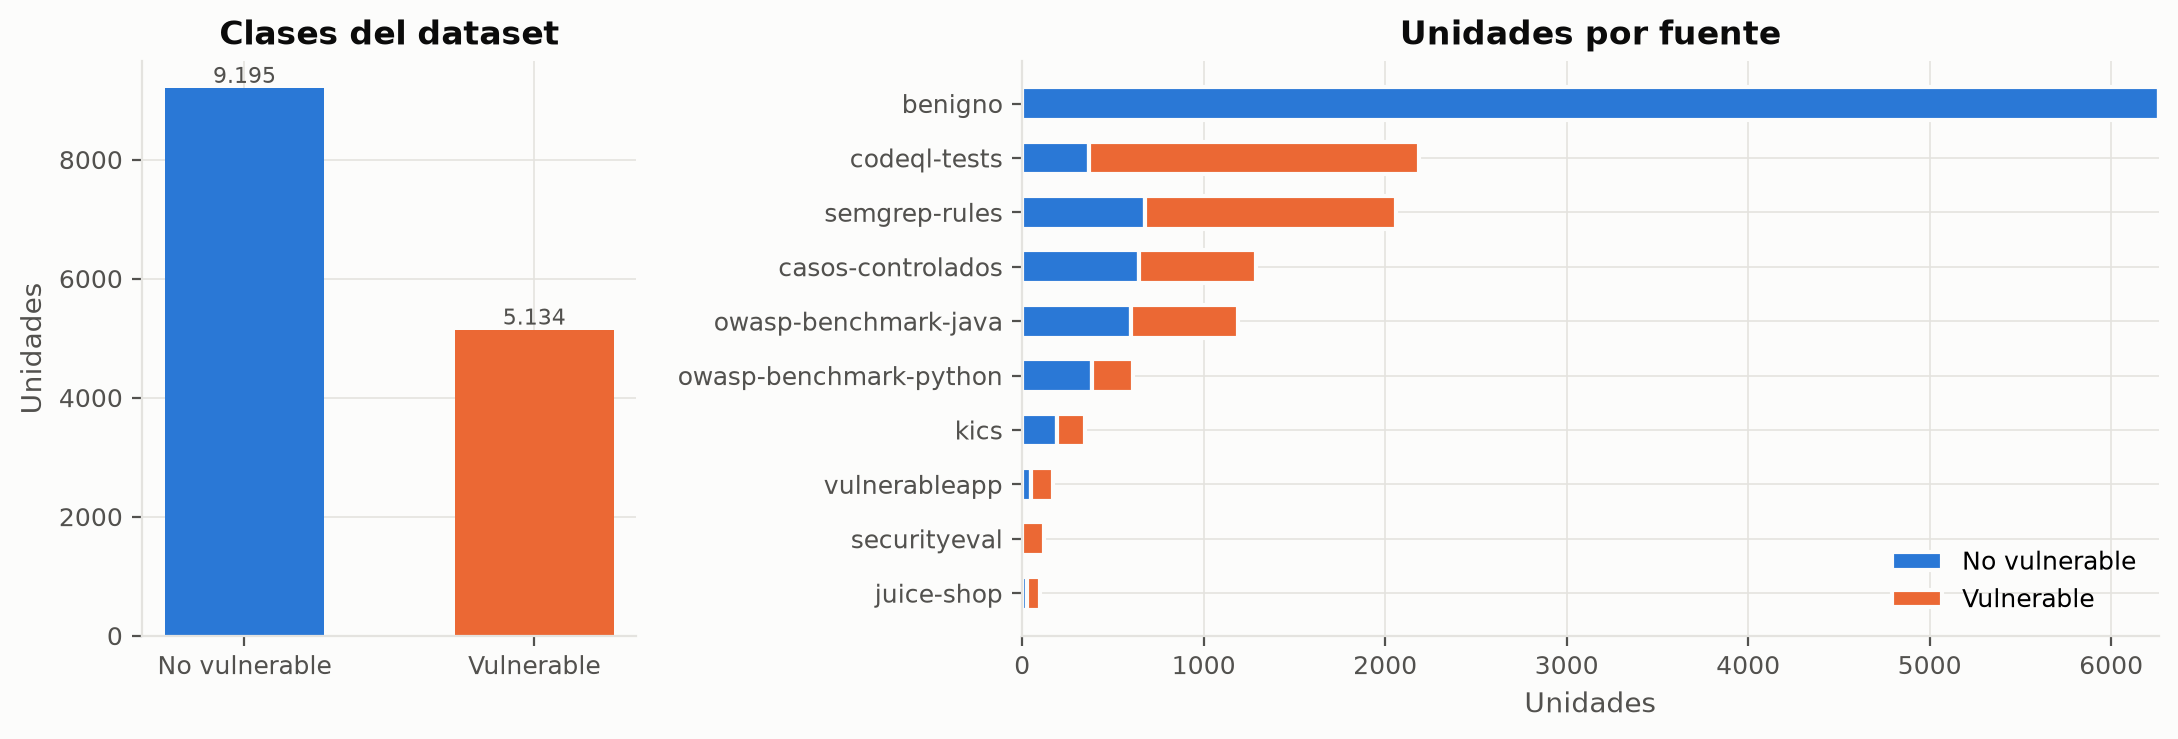
\includegraphics[width=\textwidth]{eda_clases_fuentes.png}
\caption{Proporción de clases y composición por fuente.}
\label{fig:clases}
\end{figure}

\textbf{Proporción de clases.} Hay aproximadamente dos unidades no vulnerables por cada vulnerable (Figura~\ref{fig:clases}), lo que es realista: la mayor parte del código de un proyecto no es vulnerable.

\begin{figure}[H]
\centering
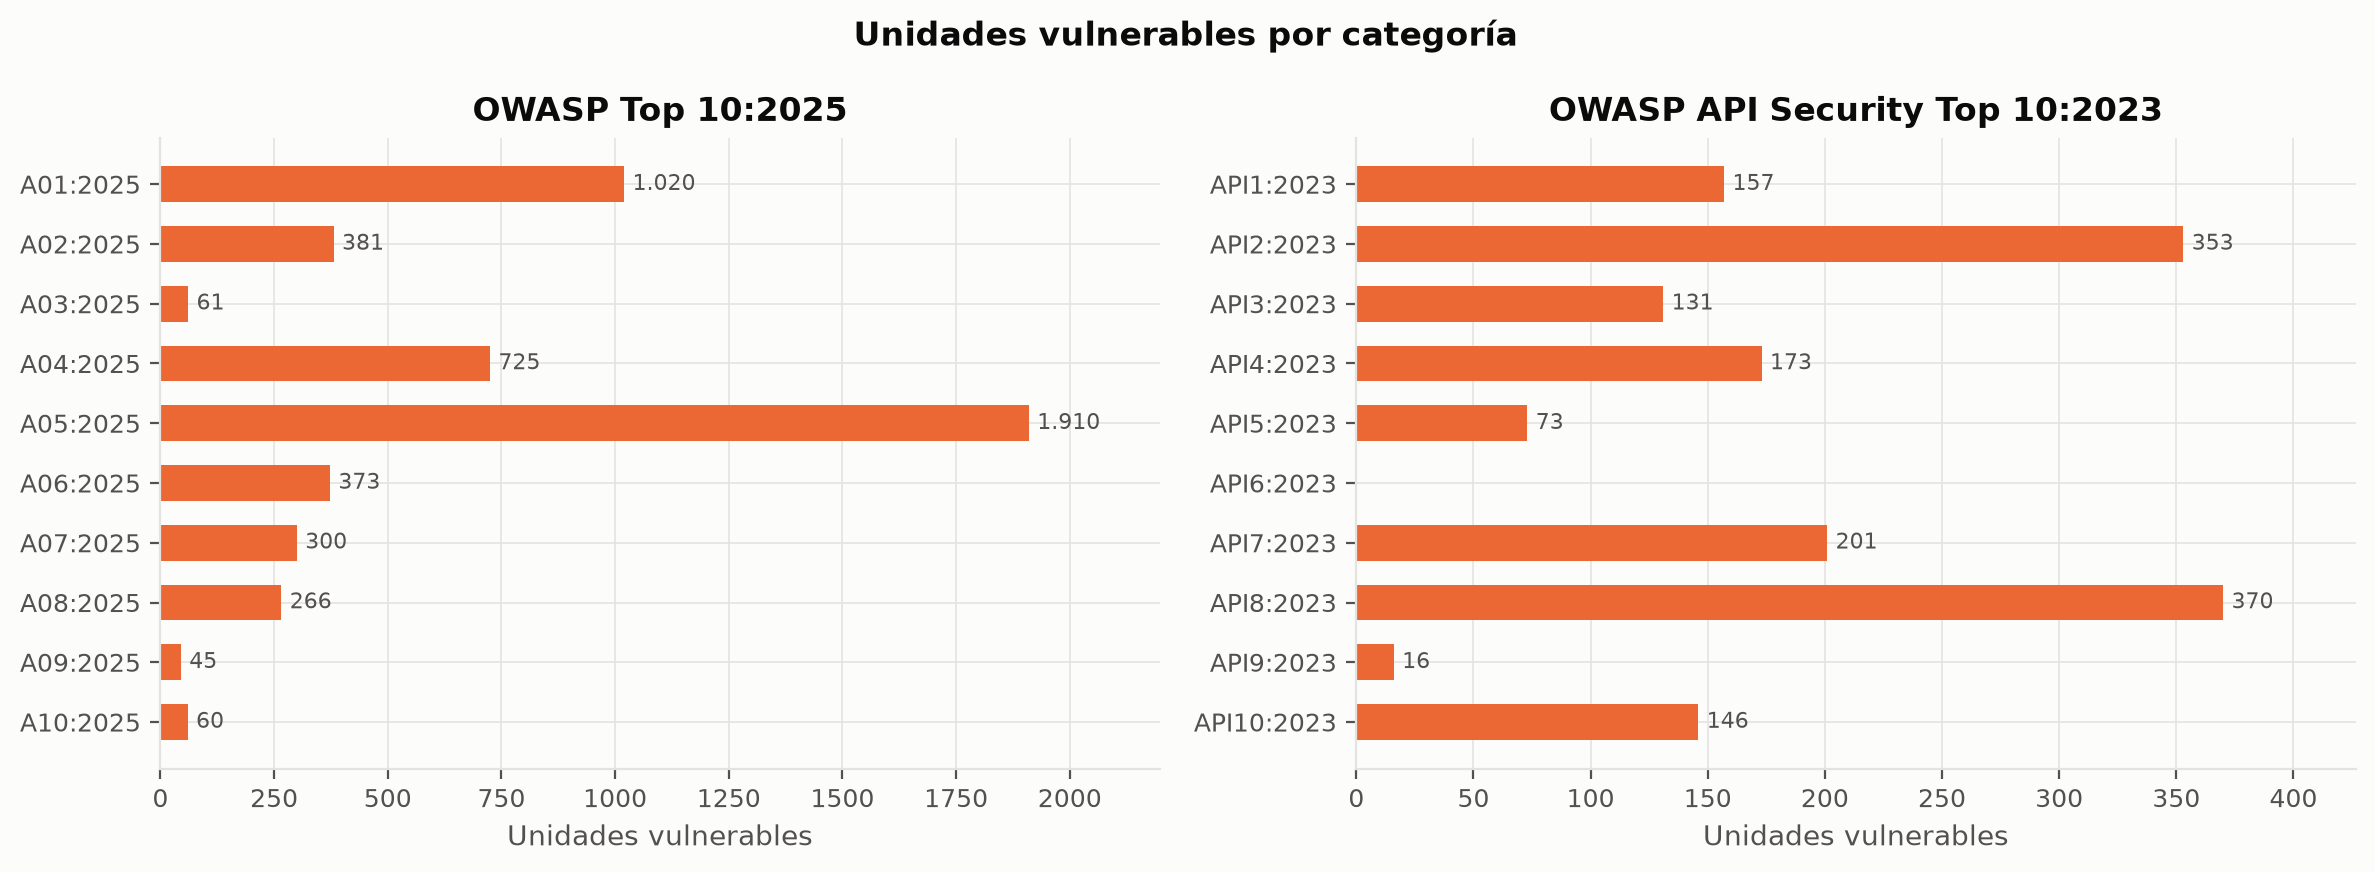
\includegraphics[width=\textwidth]{eda_categorias.png}
\caption{Distribución de las unidades vulnerables por categoría.}
\label{fig:categorias}
\end{figure}

\textbf{Distribución por categoría.} La inyección (A05), el control de acceso (A01) y la criptografía (A04) son las categorías más representadas (Figura~\ref{fig:categorias}), porque son las más estudiadas por las herramientas de análisis. A03, A09, A10, API5 y API9 tienen pocos ejemplos, y API6 no tiene ninguno: los flujos de negocio sensibles dependen de la lógica de cada aplicación y no de un patrón de código. La diferencia entre la categoría más frecuente y la menos frecuente supera dos órdenes de magnitud.

\begin{figure}[H]
\centering
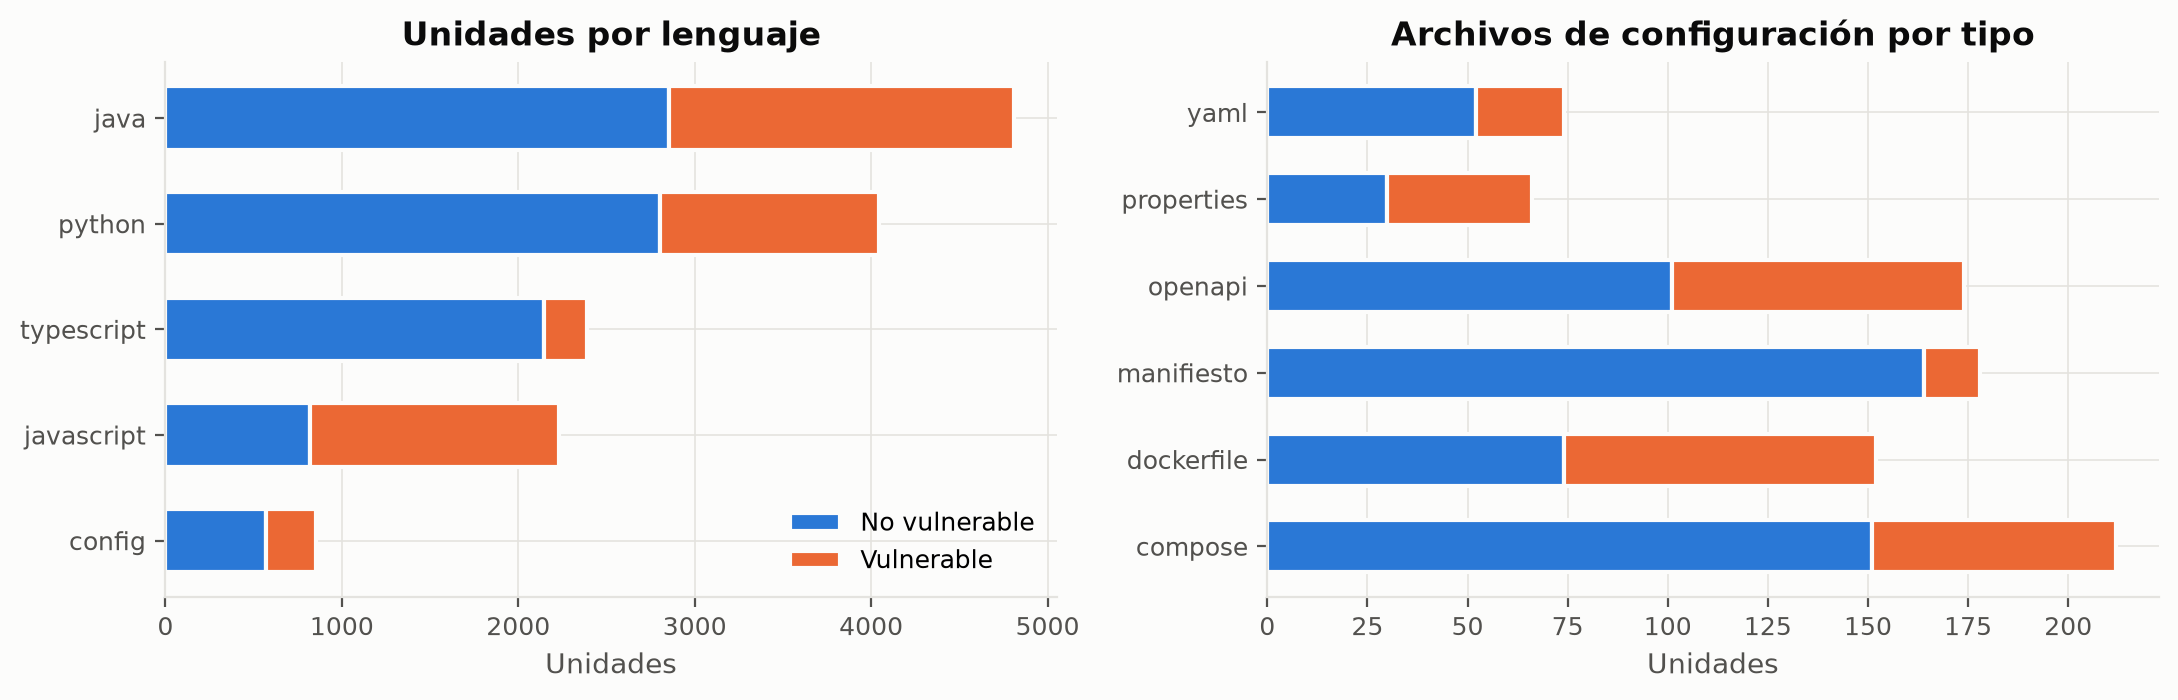
\includegraphics[width=0.95\textwidth]{eda_lenguajes.png}
\caption{Unidades por lenguaje y por tipo de archivo de configuración.}
\label{fig:lenguajes}
\end{figure}

\textbf{Lenguajes.} Los cuatro lenguajes del alcance están representados (Figura~\ref{fig:lenguajes}). La configuración es la parte menos representada.

\begin{figure}[H]
\centering
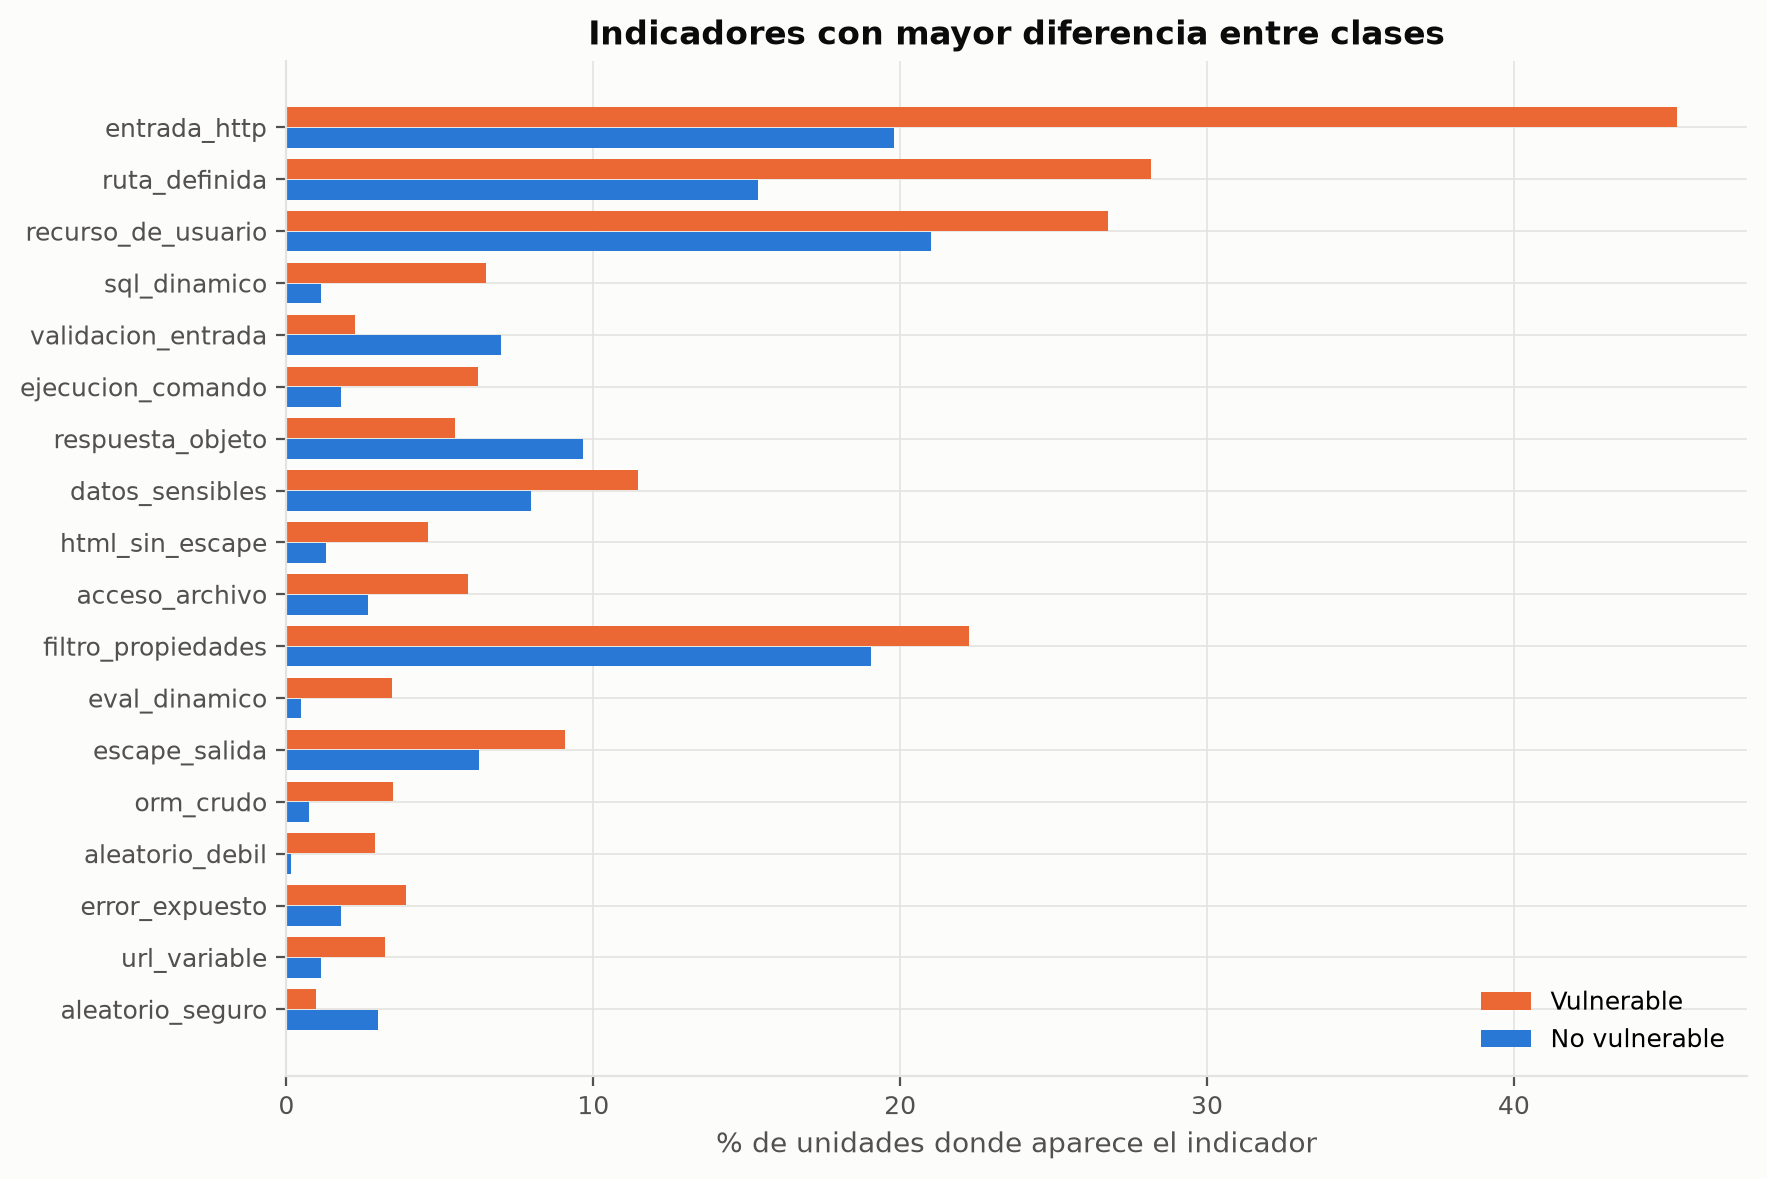
\includegraphics[width=0.8\textwidth]{eda_indicadores.png}
\caption{Indicadores de seguridad con mayor diferencia de prevalencia entre clases.}
\label{fig:indicadores}
\end{figure}

\textbf{Patrones frecuentes.} Las fuentes de entrada no confiable, las consultas SQL dinámicas, la ejecución de comandos y el hash débil son mucho más frecuentes en el código vulnerable; la validación de entrada y el uso de la identidad del usuario lo son en el no vulnerable (Figura~\ref{fig:indicadores}). Ningún indicador separa las clases por sí solo, lo que justifica un modelo que aprenda sus combinaciones.

\textbf{Calidad.} Tras la limpieza no hay duplicados, valores faltantes ni etiquetas inconsistentes. Las unidades vulnerables son algo más cortas en promedio porque muchas provienen de pruebas de reglas. Por eso la representación usa TF-IDF normalizado y la evaluación final incluye proyectos completos.

% =========================================================
\section{Fase 3. Modify: preparación y transformación}
\subsection{Representación}
Cada unidad se transforma con un pipeline de scikit-learn que se ajusta \textbf{solo con la partición de entrenamiento} y se serializa con el modelo:

\begin{enumerate}
  \item \textbf{TF-IDF de tokens} (\dimTokens{} términos, unigramas y bigramas): tokens propios de código (identificadores, operadores y marcadores como \cod{+}, \cod{\$\{} o \cod{\%}) y sub-tokens de identificadores compuestos (\cod{userId} \(\rightarrow\) \cod{user}, \cod{id}).
  \item \textbf{TF-IDF de n-gramas de caracteres} (\dimCaracteres{} n-gramas de 3 a 5 caracteres), que capta diferencias finas como \cod{execute(sql + x)} frente a \cod{execute(sql, (x,))}.
  \item \textbf{\nCaracteristicas{} características de seguridad} escaladas a \([-1, 1]\).
\end{enumerate}

\subsection{Características de seguridad}
Las características cubren las nueve familias sugeridas en el enunciado (Tabla~\ref{tab:caracteristicas}). Hay \nIndicadores{} indicadores de análisis estático; cada uno reconoce un patrón sintáctico en Java, Python, JavaScript, TypeScript o en archivos de configuración. A ellos se suman \nDerivadas{} \textbf{interacciones}, que expresan la relación entre una fuente de entrada y una operación peligrosa o la ausencia de un control (por ejemplo, \emph{ruta con identificador + búsqueda por id + sin verificación del propietario}), métricas de código y el tipo de unidad. Ningún indicador asigna una categoría OWASP: son variables cuyo peso aprende el modelo.

\begin{table}[H]
\centering\footnotesize
\caption{Características de seguridad por familia.}
\label{tab:caracteristicas}
\begin{tabularx}{\textwidth}{@{}P{4.2cm}Y@{}}
\toprule
\textbf{Característica sugerida} & \textbf{Indicadores implementados (ejemplos)}\\
\midrule
Consultas dinámicas a bases de datos & SQL concatenado o interpolado, SQL parametrizado, consultas nativas del ORM, NoSQL con datos de la petición, búsqueda por id, colección sin paginar\\
Autenticación y autorización & guards (\cod{@UseGuards}, \cod{@PreAuthorize}, \cod{Depends(get\_current\_user)}), endpoint público, verificación de rol, identidad del usuario, verificación de propietario\\
Validación de parámetros & DTO y anotaciones de validación, conversión de tipos, listas blancas, normalización de rutas, codificación de salida\\
Funciones criptográficas & hash débil, cifrado débil, aleatorio no criptográfico, hash de contraseñas robusto, TLS sin verificar, HTTP sin cifrar\\
Errores y excepciones & excepción silenciada o genérica, error expuesto al cliente, fallo abierto, registro de datos sensibles\\
Configuración de permisos y seguridad & depuración activa, CORS permisivo, CSRF deshabilitado, Actuator expuesto, contenedor privilegiado, imagen sin versión, cabeceras de seguridad\\
Tokens y credenciales & uso de JWT, JWT sin verificar, secreto literal, secreto en variables de entorno, contraseña en texto plano, límite de intentos\\
Rutas y endpoints REST & definición de ruta, identificador en la ruta, método de modificación, ruta administrativa, versión de la API, ruta de autenticación\\
Dependencias y componentes externos & peticiones salientes, URL variable, tiempo de espera, respuesta externa usada sin validar, paquetes sin versión, descargas remotas\\
\bottomrule
\end{tabularx}
\end{table}

\subsection{Variante de la representación}
Comparé cuatro variantes del bloque de seguridad: los indicadores como \(\log(1 + \text{conteo})\) o como presencia (0/1), con o sin métricas de estilo del código (cantidad de cadenas, llamadas, condicionales, profundidad). Las elegí con el conjunto de desarrollo y no con la validación (Tabla~\ref{tab:variantes}). La validación prefería una variante con métricas de estilo, pero en las aplicaciones reales las variantes con estilo quedaron por detrás: el estilo separa \emph{fuentes} de datos (el código de producción tiene más condicionales que las pruebas de reglas) más que vulnerabilidades. La variante elegida fue \emph{\variante}.

\begin{table}[H]
\centering\footnotesize
\caption{Selección de la variante de la representación (regresión logística de referencia). FA: falsas alarmas.}
\label{tab:variantes}
\begin{tabular}{@{}lccccc@{}}
\toprule
 & & \textbf{Validación} & \multicolumn{3}{c}{\textbf{Desarrollo}}\\
\cmidrule(lr){3-3}\cmidrule(l){4-6}
\textbf{Variante} & \textbf{Peso} & \textbf{AP} & \textbf{AP} & \textbf{AUC} & \textbf{Sens. (5\,\% FA)}\\
\midrule
\tabla{tabla_variantes.tex}
\bottomrule
\end{tabular}
\end{table}

\subsection{Tratamiento del desbalance}
Entre clases usé pesos balanceados y umbrales de decisión calibrados. Entre categorías usé un clasificador uno-contra-el-resto con pesos balanceados, un umbral propio por categoría y un mínimo de 15 ejemplos de entrenamiento para considerar evaluable una categoría. No usé sobremuestreo sintético: interpolar vectores TF-IDF no produce código plausible, y los casos controlados ya aportan ejemplos de las categorías escasas.

% =========================================================
\section{Fase 4. Model: construcción del modelo}
\subsection{Algoritmos comparados}
Comparé cuatro algoritmos de clasificación supervisada, todos con pesos de clase balanceados:

\begin{itemize}
  \item \textbf{Regresión logística} (\cod{C} \(\in\) \{2, 8, 32, 128\}): lineal, adecuada para matrices dispersas de alta dimensión y con coeficientes interpretables.
  \item \textbf{SVM lineal} con calibración sigmoide (\cod{C} \(\in\) \{0,2; 1; 4\}).
  \item \textbf{Random Forest} de 400 árboles sobre las \(k\) variables con mayor \(\chi^2\) (\(k\) \(\in\) \{3000, 8000\}, \cod{min\_samples\_leaf} \(\in\) \{1, 2\}).
  \item \textbf{Gradient Boosting} (HistGradientBoosting) sobre 200 componentes SVD (\cod{learning\_rate} \(\in\) \{0,05; 0,1\}, \cod{max\_leaf\_nodes} \(\in\) \{31, 63\}).
\end{itemize}
Cada configuración se probó con dos pesos para el bloque de características de seguridad (1 y 3). Los hiperparámetros se eligieron en \textbf{validación}; la prueba no participó en ninguna decisión.

\subsection{Comparación experimental}
Para el detector usé como criterio la \textbf{precisión promedio} (AP, área bajo la curva precisión--sensibilidad), que no depende del umbral y es adecuada con clases desbalanceadas. Dentro de cada algoritmo apliqué una regla de parsimonia: entre las configuraciones a menos de 0,01 de la mejor AP, elegí la más regularizada. La Tabla~\ref{tab:detector} muestra la configuración elegida de cada algoritmo; las columnas de prueba se calcularon con cada modelo entrenado solo con la partición de entrenamiento.

\begin{table}[H]
\centering\footnotesize
\caption{Comparación del detector (configuración elegida de cada algoritmo).}
\label{tab:detector}
\begin{tabularx}{\textwidth}{@{}lYccccc@{}}
\toprule
 & & \multicolumn{3}{c}{\textbf{Validación}} & \multicolumn{2}{c}{\textbf{Prueba}}\\
\cmidrule(lr){3-5}\cmidrule(l){6-7}
\textbf{Algoritmo} & \textbf{Hiperparámetros} & \textbf{AP} & \textbf{AUC} & \textbf{F1} & \textbf{F1} & \textbf{AUC}\\
\midrule
\tabla{tabla_detector.tex}
\bottomrule
\end{tabularx}
\end{table}

\begin{figure}[H]
\centering
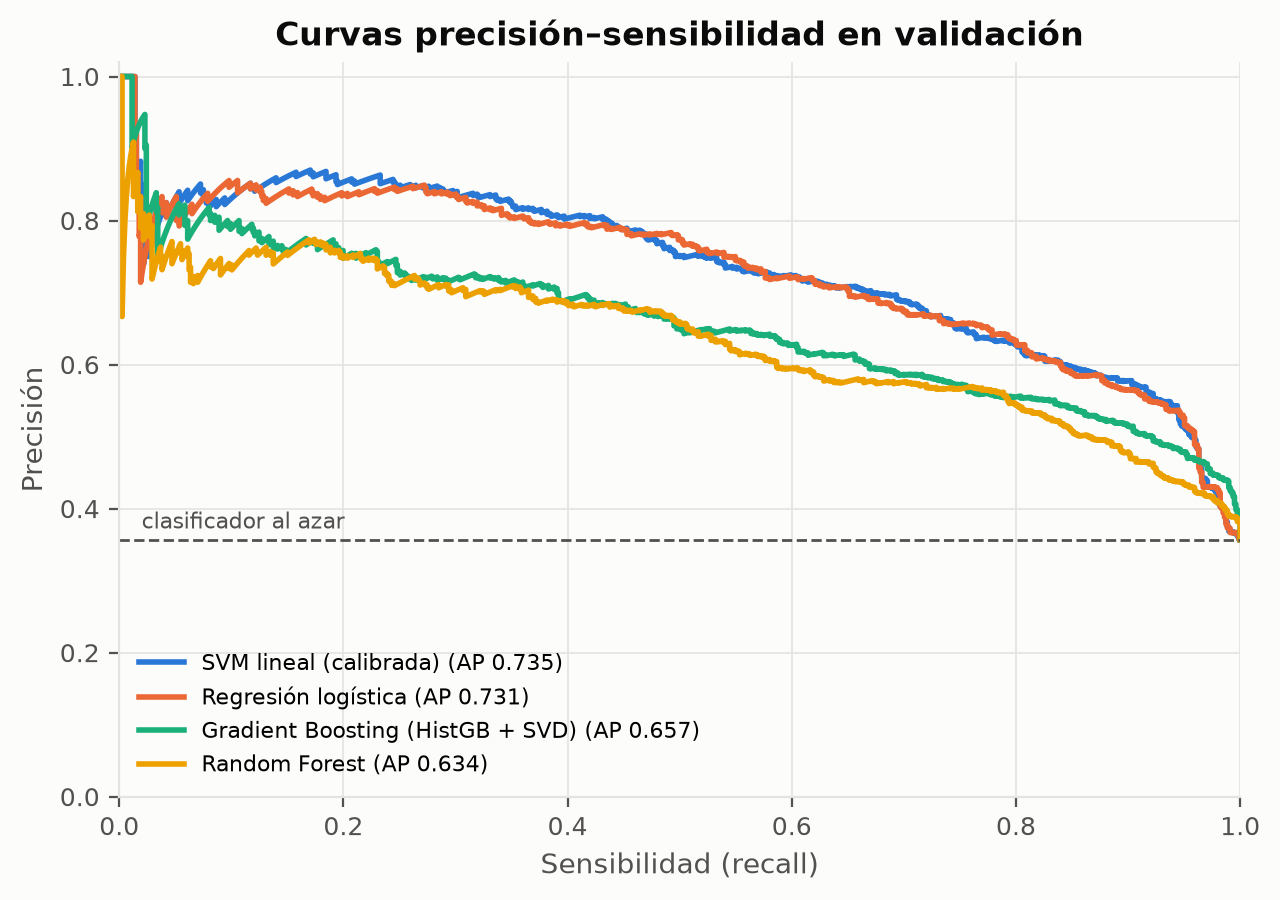
\includegraphics[width=0.62\textwidth]{modelo_curvas_pr.png}
\caption{Curvas precisión--sensibilidad de los cuatro algoritmos en validación.}
\label{fig:curvas}
\end{figure}

Para las categorías entrené cada algoritmo en modo uno-contra-el-resto sobre las unidades vulnerables y usé como criterio el \textbf{F1 macro}, que da el mismo peso a las categorías escasas que a la inyección (Tabla~\ref{tab:categorizador}).

\begin{table}[H]
\centering\small
\caption{Comparación del clasificador multietiqueta de categorías (validación).}
\label{tab:categorizador}
\begin{tabular}{@{}lccc@{}}
\toprule
\textbf{Algoritmo} & \textbf{F1 micro} & \textbf{F1 macro} & \textbf{F1 macro (umbral 0,5)}\\
\midrule
\tabla{tabla_categorizador.tex}
\bottomrule
\end{tabular}
\end{table}

\subsection{Selección y justificación}
Seleccioné la \textbf{\detAlgoritmo} (C = \detC, peso \pesoSeguridad{} para las características de seguridad) como detector y la \textbf{\catAlgoritmo} como clasificador de categorías:
\begin{itemize}
  \item La SVM lineal obtuvo la mayor precisión promedio en validación, prácticamente empatada con la regresión logística, y la regresión logística obtuvo el mayor F1 macro de categorías.
  \item Los modelos lineales aprovechan la representación dispersa completa. Random Forest y Gradient Boosting necesitan reducirla (\(\chi^2\) o SVD) y pierden información léxica fina; además quedaron por detrás en ambas tareas.
  \item Ambos producen probabilidades (la SVM mediante calibración), necesarias para el umbral y para informar la confianza.
  \item Son interpretables, y entrenan y predicen lo bastante rápido como para analizar proyectos completos en segundos.
\end{itemize}

El clasificador de CWE es una regresión logística multinomial sobre los \nClasesCWE{} CWE con al menos 10 ejemplos de entrenamiento; se usa para la descripción y la recomendación del hallazgo, y solo se informa si es coherente con las categorías asignadas. Cada categoría tiene su propio umbral, el que maximiza F1 en validación.

\textbf{Umbral operativo.} Para el detector elegí el menor umbral que deja como máximo un 5\,\% de falsas alarmas en los proyectos limpios del conjunto de desarrollo, sin superar el umbral de máximo F1 en validación. El resultado fue \umbral{} (sensibilidad \devSensibilidad{} y \devFA{} de falsas alarmas en desarrollo). Un hallazgo sin categoría (\emph{pendiente de revisión}) debe superar además el umbral de validación, porque en ese caso ni el detector ni el categorizador tienen evidencia clara.

Finalmente, reentrené los tres componentes con entrenamiento y validación, y los serialicé con su pipeline en \ruta{vulnminer/modelos/vulnminer.joblib}. La herramienta carga este archivo y no vuelve a entrenar en cada ejecución.

% =========================================================
\section{Fase 5. Assess: evaluación del modelo}
\subsection{Detector en la partición de prueba}
En la partición de prueba (\nPrueba{} unidades de grupos de origen nunca vistos), el modelo base obtuvo precisión \pruebaPrecision{}, sensibilidad \pruebaRecall{}, F1 \pruebaFUno{}, exactitud \pruebaExactitud{}, AUC-ROC \pruebaAUC{} y precisión promedio \pruebaAP{}, con una tasa de falsos positivos de \pruebaFPR{} (Figura~\ref{fig:prueba}). Con la etapa de combinación de la sección~\ref{sec:combinacion}, la decisión final de la herramienta obtuvo en la misma partición precisión \finalPrecision{}, sensibilidad \finalRecall{} y F1 \finalF{}.

\begin{figure}[H]
\centering
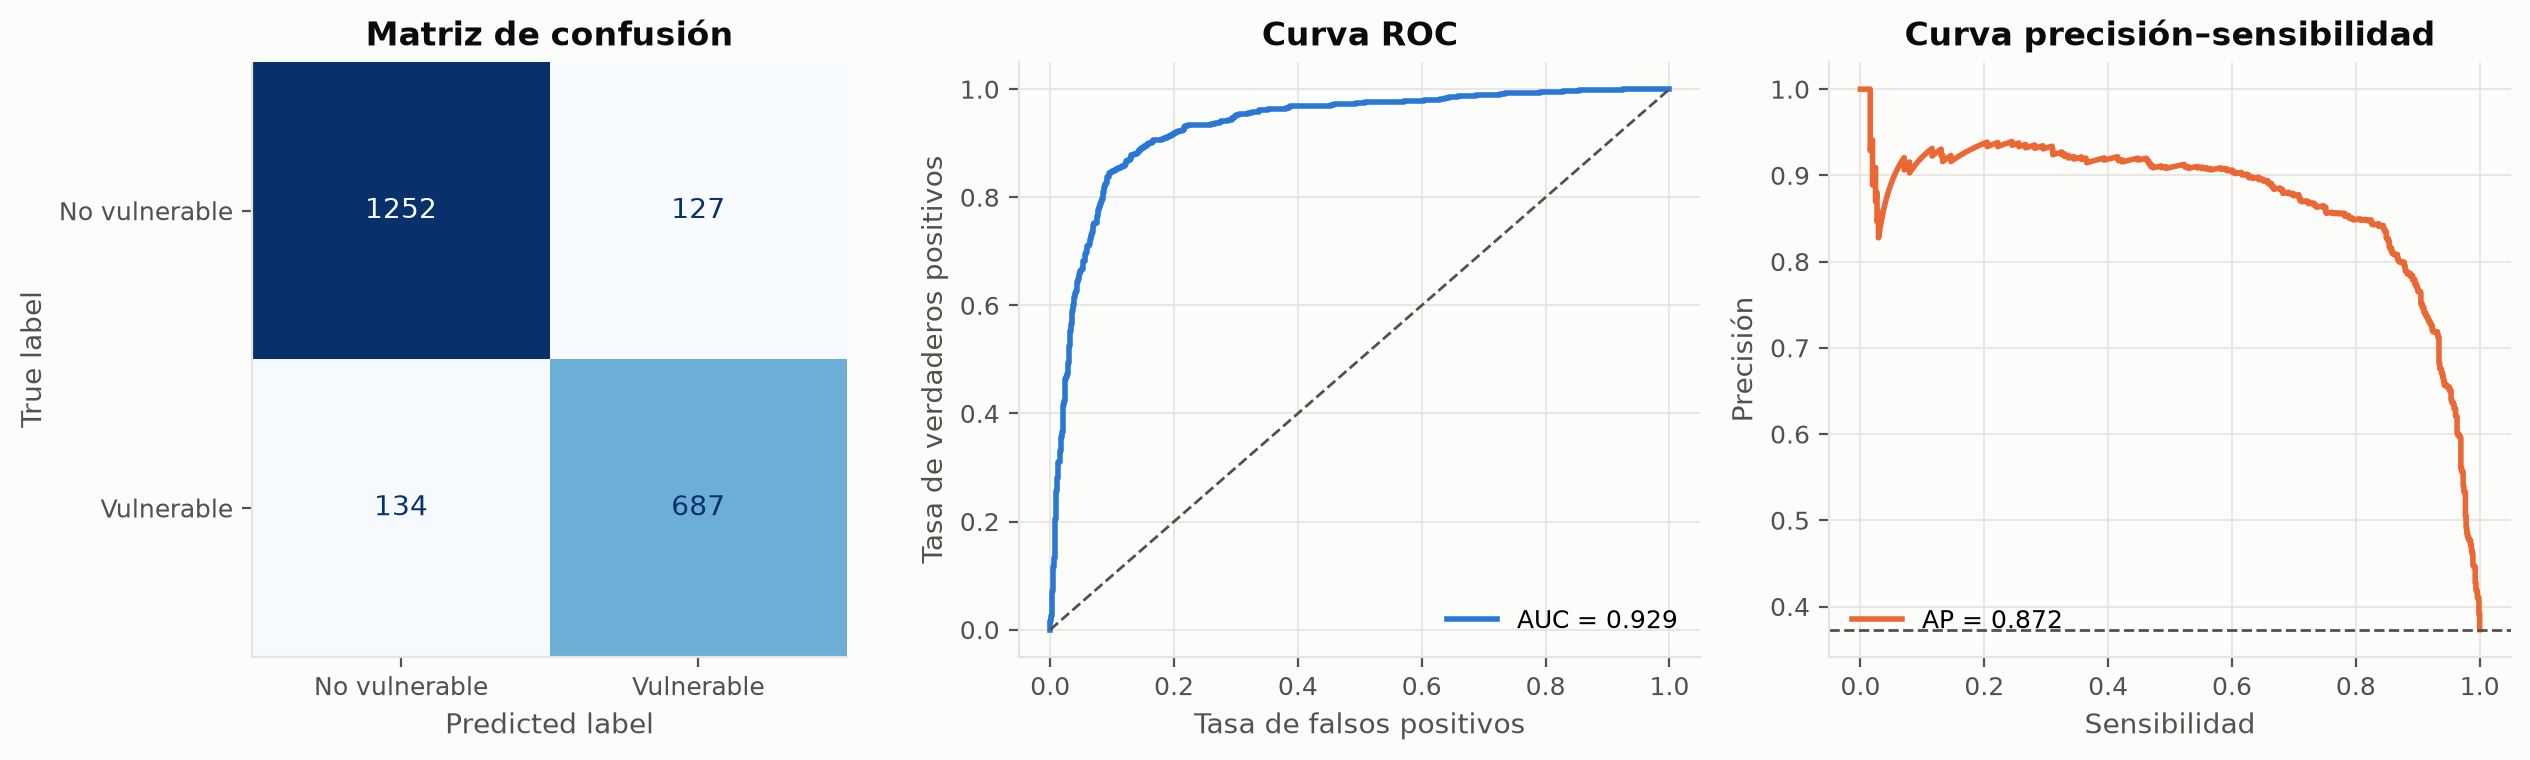
\includegraphics[width=\textwidth]{evaluacion_prueba.png}
\caption{Matriz de confusión y curvas ROC y precisión--sensibilidad del modelo base en la partición de prueba.}
\label{fig:prueba}
\end{figure}

\subsection{Desempeño por categoría}
La Tabla~\ref{tab:porcategoria} muestra dos vistas. En la vista \emph{extremo a extremo}, la unidad debe detectarse como vulnerable y además recibir la categoría correcta; es lo que experimenta quien usa la herramienta. En la vista \emph{dado que es vulnerable} se evalúa el categorizador por sí solo. En prueba, el F1 micro fue \catMicro{} y el F1 macro \catMacro{} (dado que es vulnerable), y \catMicroEE{} y \catMacroEE{} extremo a extremo. La exactitud del CWE fue \cweExactitud{}.

{\footnotesize
\setlength{\tabcolsep}{4pt}
\begin{longtable}{@{}lP{4.3cm}ccccc@{}}
\caption{Métricas por categoría en la partición de prueba (F1: extremo a extremo / dado que es vulnerable).}\label{tab:porcategoria}\\
\toprule
\textbf{Código} & \textbf{Categoría} & \textbf{Entren.} & \textbf{Prueba} & \textbf{Prec.} & \textbf{Sens.} & \textbf{F1}\\
\midrule
\endfirsthead
\toprule
\textbf{Código} & \textbf{Categoría} & \textbf{Entren.} & \textbf{Prueba} & \textbf{Prec.} & \textbf{Sens.} & \textbf{F1}\\
\midrule
\endhead
\tabla{tabla_categorias.tex}
\bottomrule
\end{longtable}
}

\begin{figure}[H]
\centering
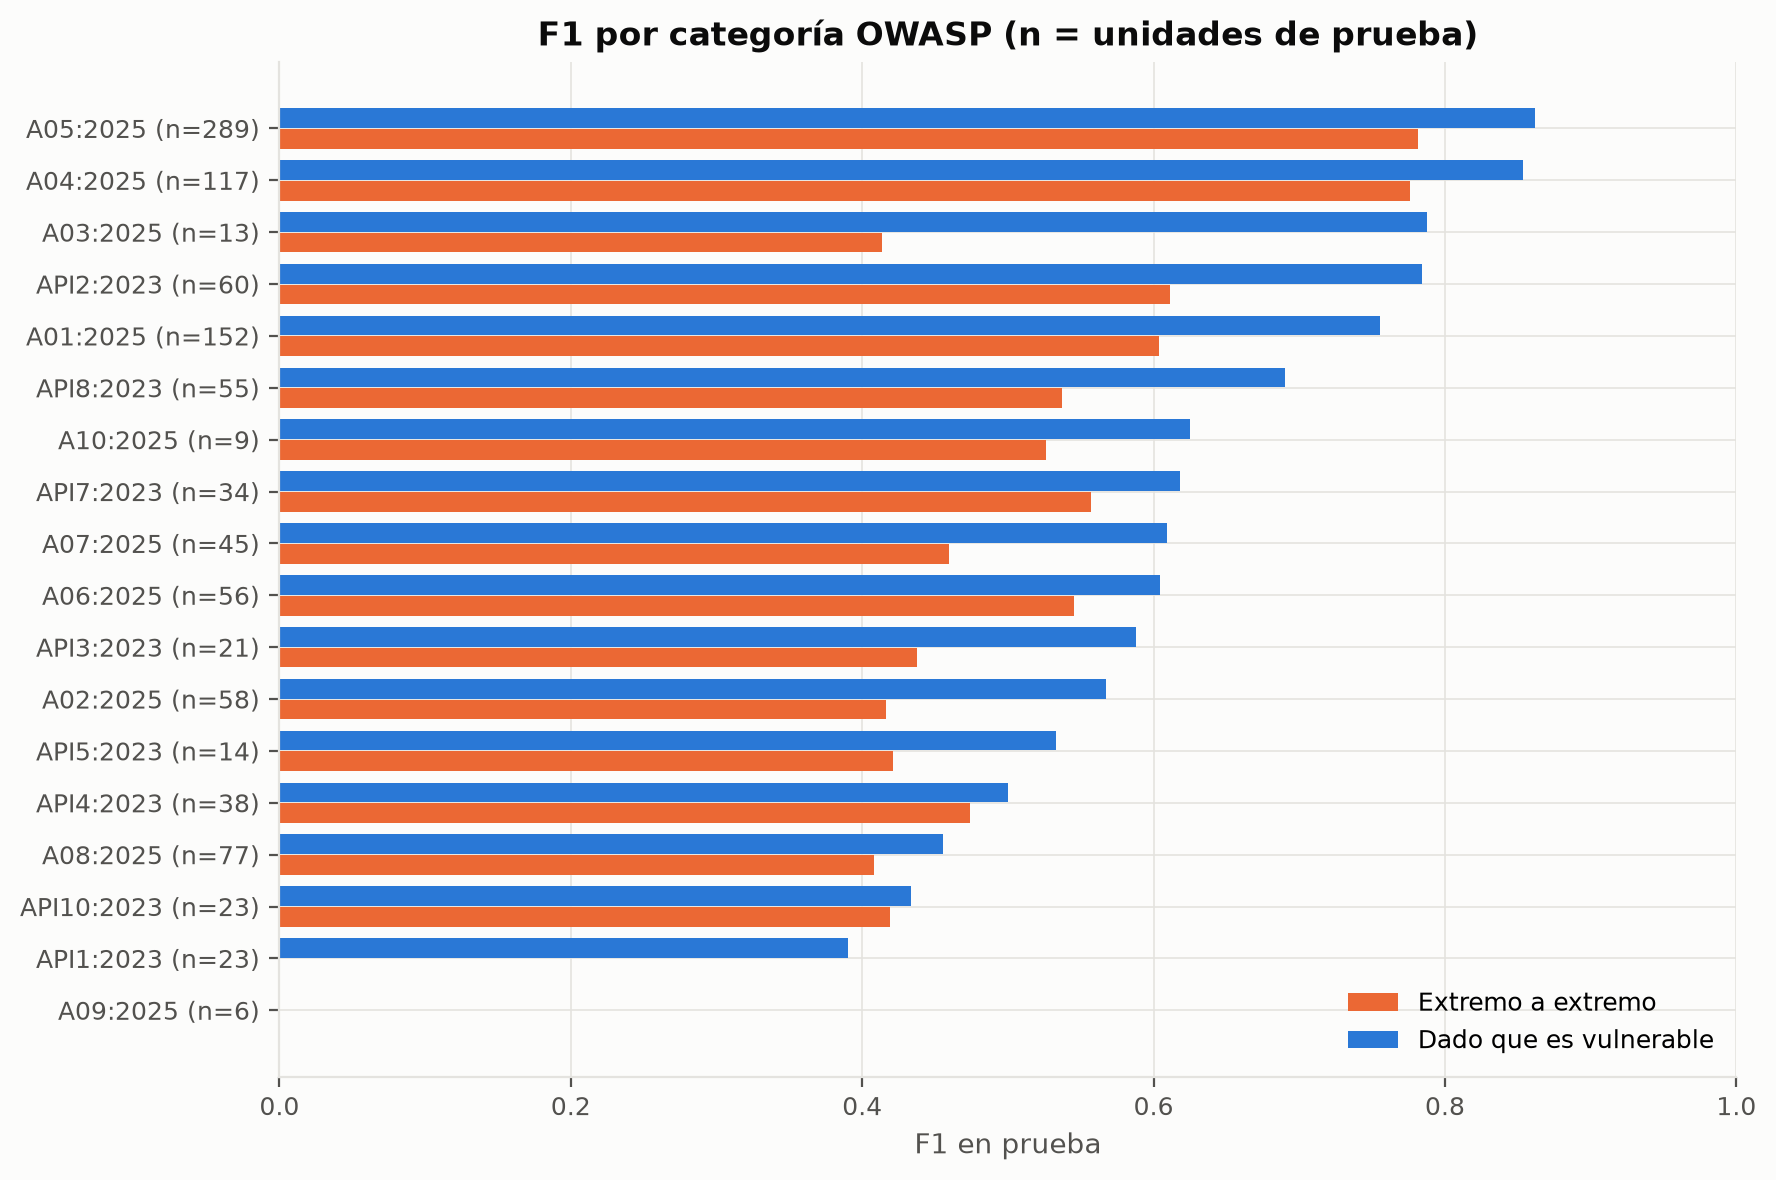
\includegraphics[width=0.85\textwidth]{evaluacion_categorias.png}
\caption{F1 por categoría en la partición de prueba.}
\label{fig:fcategorias}
\end{figure}

Las categorías con F1 bajo son las que tienen pocos ejemplos en la prueba (A09, A10) o las de autorización (API1, API5), en las que la versión vulnerable y la segura se diferencian por una comprobación ausente.

\subsection{Análisis de falsos positivos y falsos negativos}
Revisé uno por uno los errores del detector en la partición de prueba (notebook \ruta{05_assess.ipynb}, sección~3) y los agrupé por su causa.

\textbf{Falsos positivos.} La mayoría proviene de las pruebas de CodeQL y del OWASP Benchmark para Java. En estas fuentes, la versión segura de un caso suele diferir de la vulnerable en un detalle que no está en la propia función: un valor que se reemplaza por una constante dentro de una condición que siempre se cumple, un saneamiento aplicado en otro método o una lista blanca definida en otra clase. Para un modelo que observa la función, ambas versiones tienen la misma fuente de entrada y la misma operación peligrosa. En cambio, en el código de los proyectos reales sin vulnerabilidades, la tasa de falsos positivos fue de apenas \benignoFPR{}, lo que indica que el modelo no confunde el código de producción común con código vulnerable.

\textbf{Falsos negativos.} Se concentran en las categorías de autorización: A01 y, en particular, CWE-639 (acceso a un objeto ajeno por su identificador, API1). En estos casos, la vulnerabilidad es la \emph{ausencia} de una línea, como la comparación del propietario del recurso con el usuario autenticado, y la versión segura y la vulnerable comparten casi todo el texto. Le siguen la verificación de la firma del JWT (CWE-347), donde la diferencia suele ser una opción de configuración del verificador, y la deserialización insegura (CWE-502). La configuración casi no presenta errores, porque sus patrones son más regulares que los del código.

\subsection{Sobreajuste y generalización}
Sobre una muestra de los datos de ajuste (entrenamiento y validación), el modelo base obtiene F1 = \ajusteF{} y AUC = \ajusteAUC{}, frente a F1 = \pruebaFUno{} y AUC = \pruebaAUC{} en la prueba. La diferencia muestra que el modelo memoriza parte de los ejemplos, algo esperable en un modelo léxico de alta dimensión. Lo importante es cuánto conserva fuera de las fuentes de entrenamiento: en \webN{} fragmentos reales de foros y documentación oficial obtuvo F1 = \webF{} (AUC = \webAUC{}), y en proyectos completos detectó la mayor parte de las vulnerabilidades documentadas (sección~\ref{sec:proyectos}).

Para limitar el sobreajuste tomé estas decisiones: partición por grupo de origen, eliminación de las marcas de etiqueta, elección de la variante y del umbral con un conjunto de desarrollo independiente, y reglas de parsimonia que prefieren el modelo más regularizado cuando la diferencia de desempeño es pequeña. El ejemplo más claro de su utilidad es la selección de la variante: la validación habría elegido una representación con métricas de estilo, que en aplicaciones reales quedó por detrás de la elegida (Tabla~\ref{tab:variantes}).

\subsection{Contribución del modelo de clasificación}\label{sec:contribucion}
El enunciado permite apoyarse en reglas o en herramientas existentes siempre que se evidencie la contribución del modelo. Lo medí con dos experimentos (\ruta{scripts/contribucion.py}, notebook \ruta{05_assess.ipynb}, sección~6).

\textbf{Ablación.} Con el mismo algoritmo y el mismo protocolo del modelo base comparé: las reglas solas (sin aprendizaje: una unidad es vulnerable si activa al menos \(k\) indicadores de operación peligrosa); los indicadores con el clasificador (y con Random Forest, por si necesitaran un modelo no lineal); el texto solo (TF-IDF); el modelo completo; y la decisión final de la herramienta. En los proyectos externos la comparación se hizo a nivel de unidad: las \extDocumentadas{} funciones con vulnerabilidades documentadas frente a las \sgUnidadesLimpias{} unidades de dos proyectos limpios. La última columna compara todas las variantes en el mismo punto: la sensibilidad cuando se permite un 5\,\% de falsas alarmas.

\begin{table}[H]
\centering\footnotesize
\caption{Ablación del detector. FA: unidades limpias marcadas (\%).}
\label{tab:ablacion}
\begin{tabularx}{\textwidth}{@{}Ycccccccc@{}}
\toprule
 & & \multicolumn{2}{c}{\textbf{Prueba}} & \multicolumn{4}{c}{\textbf{Proyectos externos (por unidad)}}\\
\cmidrule(lr){3-4}\cmidrule(l){5-8}
\textbf{Variante} & \textbf{Variables} & \textbf{F1} & \textbf{AUC} & \textbf{Detect.} & \textbf{FA} & \textbf{AUC} & \textbf{Sens. 5\,\% FA}\\
\midrule
\tabla{tabla_ablacion.tex}
\bottomrule
\end{tabularx}
\end{table}

\begin{figure}[H]
\centering
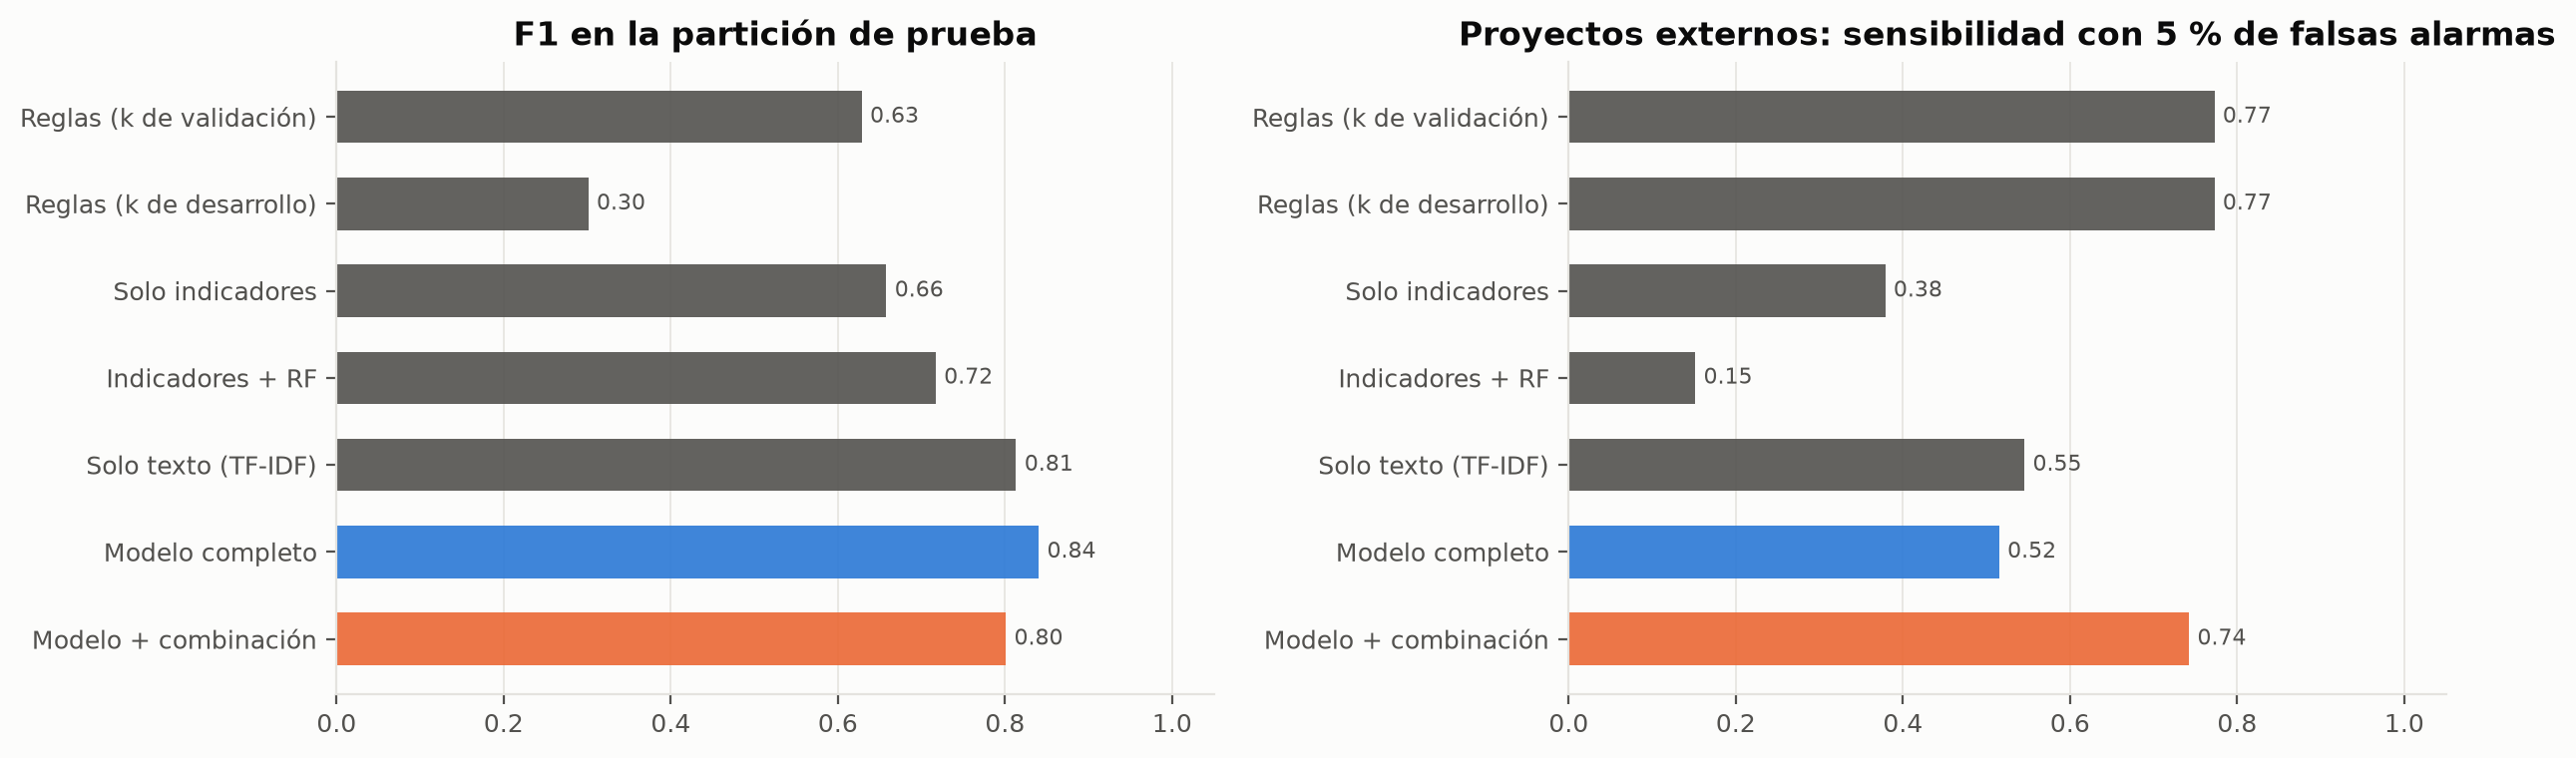
\includegraphics[width=\textwidth]{contribucion_ablacion.png}
\caption{Ablación: F1 en la prueba y sensibilidad con 5\,\% de falsas alarmas en los proyectos externos.}
\label{fig:ablacion}
\end{figure}

La ablación muestra dos cosas. En la partición de prueba, donde hay que distinguir un caso vulnerable de su versión corregida, el aprendizaje es imprescindible: con el umbral elegido en validación, las reglas solas marcan como vulnerable la mitad del código limpio, y con el umbral calibrado en desarrollo su F1 cae a \ablReglasDesarrolloF{}, frente a \ablCompletoF{} del modelo completo. En los proyectos reales, en cambio, las reglas con el umbral de desarrollo detectaron \ablReglasDesarrolloDet{} de \extDocumentadas{} vulnerabilidades, más que el modelo base (\ablCompletoDet{}). La explicación es un \textbf{cambio de distribución}: en los datos de entrenamiento, la versión vulnerable y la segura de un caso tienen casi las mismas operaciones peligrosas, por lo que el modelo aprendió a no dar peso a la \emph{cantidad} de evidencia estática; en una aplicación real, las funciones vulnerables suelen acumular varias operaciones peligrosas a la vez. Ninguna de las dos fuentes de información basta por sí sola, y eso motivó la iteración de la sección siguiente.

\subsection{Iteración: etapa de combinación}\label{sec:combinacion}
SEMMA es un proceso iterativo: la evaluación puede llevar a volver a transformar los datos o a ajustar el modelo. Con el conjunto de desarrollo, que es de aplicaciones reales, ajusté una regresión logística de dos variables: el logit de la probabilidad del modelo base (coeficiente \combCoefP{}) y la cantidad de indicadores de operación peligrosa activos (coeficiente \combCoefE{}). La decisión en el código queda así: una unidad es vulnerable si el modelo base está seguro (\(p \ge \combUbase\)) o si la probabilidad combinada supera \combUcomb{}.

Los umbrales se eligieron con predicciones fuera de pliegue (validación cruzada de cinco pliegues en el conjunto de desarrollo), manteniendo como máximo un 5\,\% de falsas alarmas: la mayor sensibilidad y, dentro de una tolerancia de una vulnerabilidad, la opción que más respeta al modelo base (Tabla~\ref{tab:combinacion}). La combinación se aplica solo al código de servidor, porque el conjunto de desarrollo no tiene vulnerabilidades de configuración ni de código de navegador; para Dockerfile, \cod{docker-compose}, YAML, manifiestos y frontend (React, Angular, Vue) decide el modelo base. La decisión sigue siendo del modelo: los indicadores son una variable más de una regresión aprendida, no una regla que asigne la etiqueta.

\begin{table}[H]
\centering\small
\caption{Selección de los umbrales de la combinación (conjunto de desarrollo, predicciones fuera de pliegue).}
\label{tab:combinacion}
\begin{tabular}{@{}cccc@{}}
\toprule
\textbf{Umbral del modelo base} & \textbf{Umbral combinado} & \textbf{Sensibilidad} & \textbf{Falsas alarmas (\%)}\\
\midrule
\tabla{tabla_combinacion.tex}
\bottomrule
\end{tabular}
\end{table}

En el conjunto de desarrollo, la sensibilidad con 5\,\% de falsas alarmas pasó de \combBaseDevSens{} a \combDevSens{}. A nivel de unidad en los proyectos externos, la herramienta detectó \ablHerramientaDet{} de \extDocumentadas{} vulnerabilidades, frente a \ablCompletoDet{} del modelo base, con menos falsas alarmas (\ablHerramientaFA{} frente a \ablCompletoFA{}). El costo es una baja del F1 en la partición de prueba (de \pruebaFUno{} a \finalF{}), que está formada mayoritariamente por casos de pruebas de reglas. Acepté ese costo porque la herramienta se usará con proyectos reales.

En estos proyectos, las reglas solas con el umbral de desarrollo quedan a un nivel similar al de la herramienta (\ablReglasDesarrolloDet{} detectadas y \ablReglasDesarrolloFA{} de falsas alarmas). Esto confirma que la cantidad de evidencia estática es una señal fuerte en aplicaciones vulnerables reales, pero las reglas no son una alternativa al modelo: en la partición de prueba su F1 cae a \ablReglasDesarrolloF{} porque no distinguen una función corregida de la vulnerable, y no asignan la categoría OWASP, el CWE ni la línea relevante. La herramienta mantiene el nivel de las reglas en aplicaciones reales y el del modelo en los casos sutiles.

\textbf{Comparación con Semgrep.} Semgrep \cite{semgreptool} es un analizador estático por reglas muy usado. Lo ejecuté (versión \sgVersion) con las reglas comunitarias de \cod{semgrep-rules} para los mismos lenguajes, sobre los mismos proyectos y con el mismo criterio de acierto: un hallazgo dentro de la función documentada. Son las mismas reglas cuyos casos de prueba forman parte del dataset, de modo que la comparación mide si el modelo generaliza más allá de las reglas de las que aprendió.

\begin{table}[H]
\centering\footnotesize
\caption{vulnminer frente a Semgrep. En los proyectos limpios se muestran las unidades marcadas.}
\label{tab:semgrep}
\begin{tabularx}{\textwidth}{@{}Yccccc@{}}
\toprule
 & & \multicolumn{2}{c}{\textbf{Detectadas / marcadas}} & \multicolumn{2}{c}{\textbf{Hallazgos}}\\
\cmidrule(lr){3-4}\cmidrule(l){5-6}
\textbf{Proyecto} & \textbf{Doc.} & \textbf{Semgrep} & \textbf{vulnminer} & \textbf{Semgrep} & \textbf{vulnminer}\\
\midrule
\tabla{tabla_semgrep.tex}
\bottomrule
\end{tabularx}
\end{table}

\begin{figure}[H]
\centering
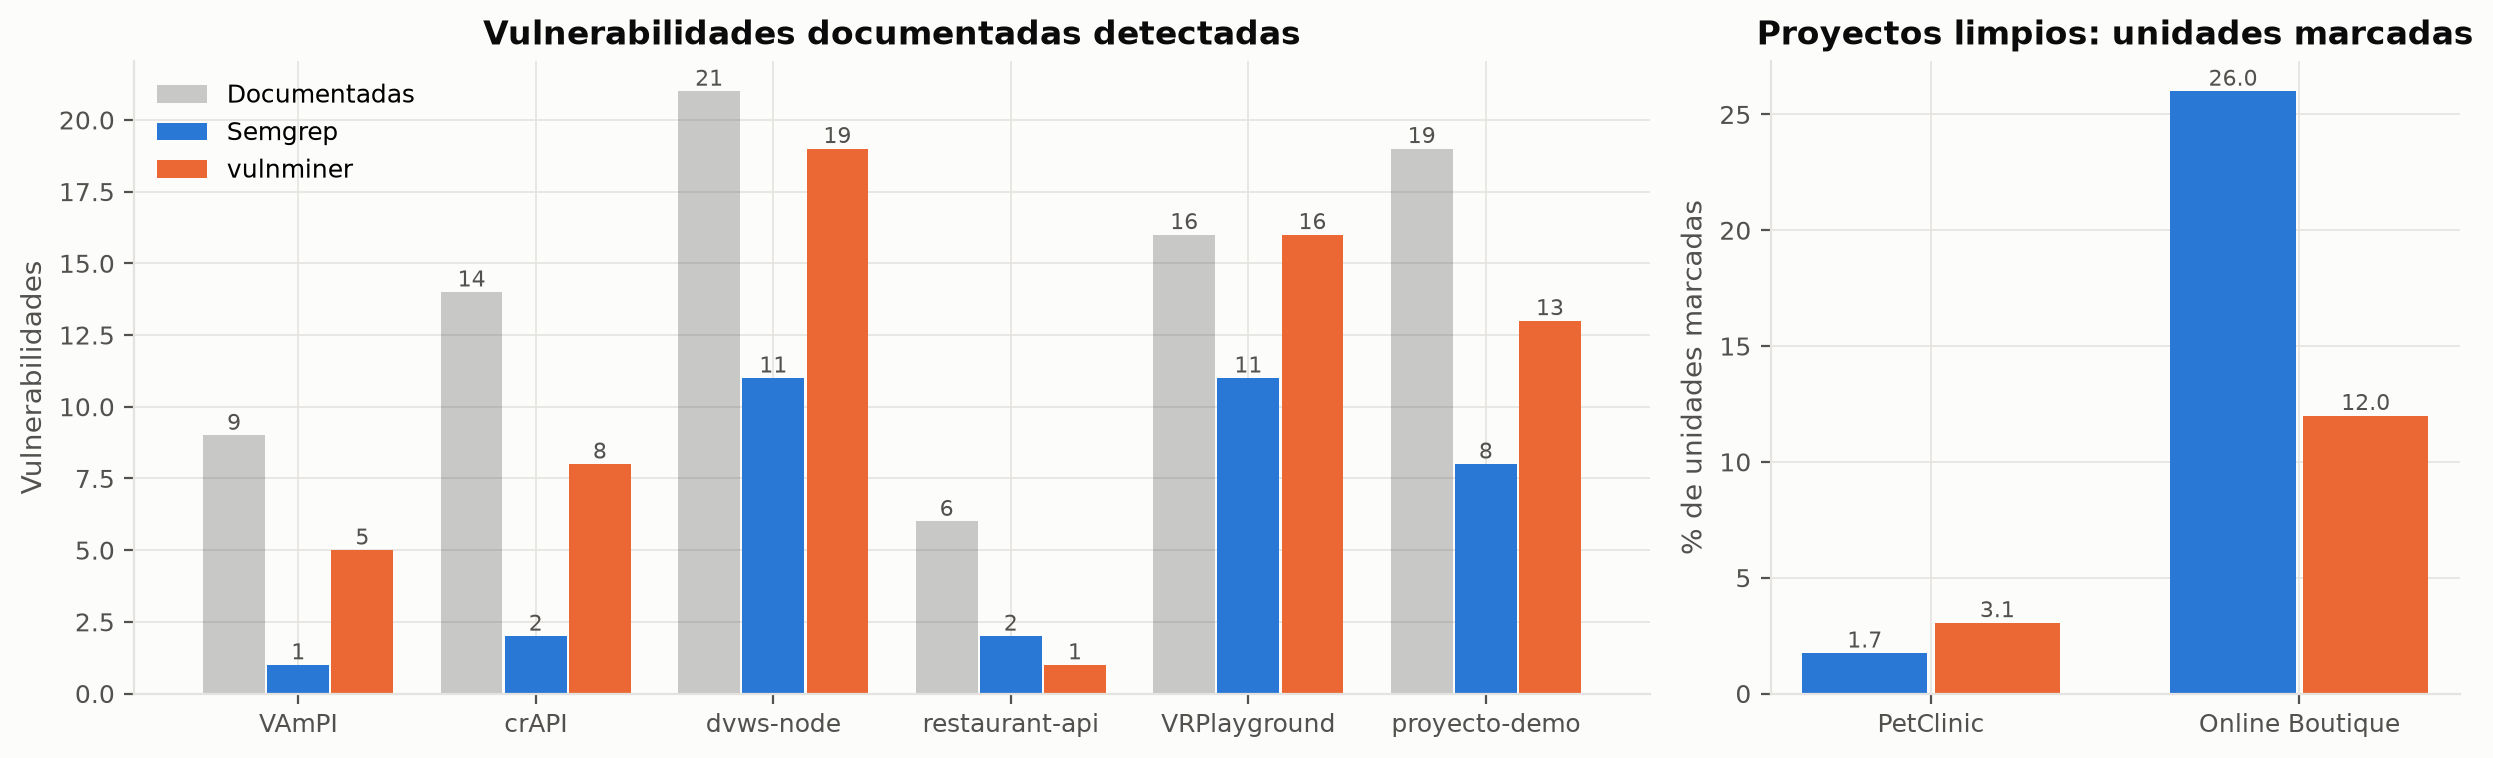
\includegraphics[width=\textwidth]{contribucion_semgrep.png}
\caption{Vulnerabilidades documentadas detectadas y unidades marcadas en proyectos limpios: vulnminer frente a Semgrep.}
\label{fig:semgrep}
\end{figure}

vulnminer detectó \sgVulnminer{} de \extDocumentadas{} vulnerabilidades documentadas y Semgrep \sgDetectadas{}. Ambas herramientas coincidieron en \sgAmbas{}; vulnminer encontró \sgSoloVulnminer{} que Semgrep no encontró, y Semgrep \sgSoloSemgrep{} que vulnminer no encontró. En los proyectos limpios, vulnminer marcó en total \sgMarcadasVm{} unidades de \sgUnidadesLimpias{} y Semgrep \sgMarcadas{}: Semgrep marcó menos en PetClinic, y vulnminer bastante menos en Online Boutique. Las que solo encontró vulnminer se concentran en autenticación y manejo de JWT (API2), consumo ilimitado de recursos (API4) y asignación masiva, para las que las reglas genéricas no tienen patrones y el modelo sí los aprendió de los casos controlados; también incluyen inyecciones escritas de formas que las reglas no reconocen (XPath, LDAP, NoSQL y plantillas). Las dos herramientas son complementarias: su unión cubre \sgUnion{} de las \extDocumentadas{} vulnerabilidades.

% =========================================================
\section{Herramienta CLI}
\subsection{Instalación y ejecución}
La herramienta se instala como paquete de Python (versión 3.11 o superior) y se ejecuta con una única instrucción desde el directorio raíz del proyecto analizado:
\begin{lstlisting}
git clone https://github.com/Jeancarlospp/Clasificador_vulnerabilidades.git
cd Clasificador_vulnerabilidades
python3 -m venv .venv && source .venv/bin/activate
pip install .
cd ruta/al/proyecto-microservicios
vulnminer scan . --standards owasp2025,api2023 --format json,html --output ./reportes
\end{lstlisting}
Probé la instalación desde un clon limpio, en un entorno virtual nuevo, y el análisis del proyecto de demostración tardó menos de dos segundos. Además de \cod{scan}, la herramienta ofrece \cod{vulnminer fragmento} (analiza un fragmento suelto) y \cod{vulnminer info} (muestra el modelo, sus métricas y las categorías evaluadas). La opción \cod{--threshold} permite una auditoría más exhaustiva bajando el umbral del modelo base.

\subsection{Proceso de análisis}
\begin{enumerate}
  \item \textbf{Descubrimiento.} Identifica los microservicios por sus manifiestos (\cod{package.json}, \cod{pom.xml}, \cod{build.gradle}, \cod{requirements.txt}, \cod{pyproject.toml}) o su \cod{Dockerfile}, usa los nombres del \cod{docker-compose} cuando existen y reconoce las tecnologías (NestJS, Express, Spring Boot, FastAPI, Flask, Django, React, Angular, Vue). Excluye dependencias, compilados, código generado y pruebas (estas se incluyen con \cod{--include-tests}). Los lenguajes no soportados y los archivos omitidos (binarios, mayores de 1~MB o sin permiso de lectura) se informan en el reporte.
  \item \textbf{Selección de archivos.} Código Java, Python, JavaScript y TypeScript; \cod{application.yml} y \cod{.properties}; \cod{.env}; \cod{Dockerfile}; \cod{docker-compose}; especificaciones OpenAPI/Swagger; y manifiestos de dependencias.
  \item \textbf{Predicción.} Segmenta, extrae las características, aplica el pipeline y el modelo serializado con su etapa de combinación, y asigna las categorías que superan su umbral.
  \item \textbf{Localización.} Entre las líneas que más reducen la probabilidad de vulnerabilidad al quitarlas de la unidad (\emph{oclusión}), se informa la que contiene la operación peligrosa (consulta, deserialización, petición saliente) antes que la fuente de entrada. En los proyectos externos, la línea informada estuvo a tres líneas o menos de la documentada en \locTres{} de \locN{} detecciones.
  \item \textbf{Severidad y estado.} La severidad parte de la severidad base del CWE o de la categoría y se ajusta según el contexto: datos de la petición que llegan a una operación peligrosa, endpoint sin autenticación o archivo de pruebas. No se deriva de la confianza del modelo, y su justificación acompaña al hallazgo. El estado distingue entre hallazgos \emph{potenciales respaldados por evidencia estática}, los que \emph{requieren verificación manual o dinámica} (autorización, lógica de negocio, monitoreo) y los \emph{pendientes de revisión}. La herramienta nunca marca un hallazgo como confirmado, porque el análisis estático no puede confirmarlo.
  \item \textbf{Reportes.} Resumen en consola y reportes \cod{analisis.json} y \cod{analisis.html}.
\end{enumerate}

\subsection{Información de cada hallazgo}
Cada hallazgo incluye los trece elementos exigidos:
\begin{enumerate}
  \item Identificador.
  \item Microservicio.
  \item Archivo.
  \item Línea.
  \item Descripción.
  \item Evidencia técnica: fragmento con la línea resaltada, líneas que más aportan a la predicción, indicadores de análisis estático, y probabilidades del modelo base y de la combinación.
  \item Categoría del Top 10:2025.
  \item Categoría de API Security 2023.
  \item CWE.
  \item Confianza del modelo.
  \item Severidad con su justificación.
  \item Recomendación de remediación.
  \item Estado de verificación.
\end{enumerate}
El reporte HTML es autocontenido y permite examinar los resultados mediante una matriz de microservicio \(\times\) categoría y filtros por microservicio, categoría, severidad y texto. También informa las categorías no evaluadas.

\subsection{Ejemplo de salida}
Para la demostración escribí un proyecto con la estructura del enunciado (\ruta{ejemplos/proyecto-microservicios}): un \emph{API gateway} en Express, un servicio de usuarios en NestJS, uno de productos en Spring Boot y uno de pedidos en FastAPI, con un \cod{docker-compose.yml}. Los reportes completos están en \ruta{ejemplos/reporte_demo/}. Este es un extracto de la salida en consola:

\begin{lstlisting}
========================================
VULNMINER - SECURITY SCAN
========================================
Proyecto: proyecto-microservicios
Microservicios identificados: 4
Archivos analizados: 19
Unidades analizadas: 65
Hallazgos potenciales: 17
Por severidad: Crítica 2, Alta 8, Media 7, Baja 0
----------------------------------------
HALLAZGO 002
----------------------------------------
Servicio: product-service
Archivo: product-service/src/main/java/com/tienda/productos/ProductRepository.java
Linea: 22
OWASP Top 10: A05:2025
OWASP API: -
CWE: CWE-89 Improper Neutralization of Special Elements used in an SQL Command
Problema potencial:
Consulta SQL construida por concatenación o interpolación de datos (inyección SQL).
Evidencia: datos de la petición llegan a una consulta SQL construida dinámicamente.
Confianza del modelo: 0.99
Severidad estimada: Crítica
Estado: Potencial - respaldado por evidencia estática
\end{lstlisting}

\begin{figure}[H]
\centering
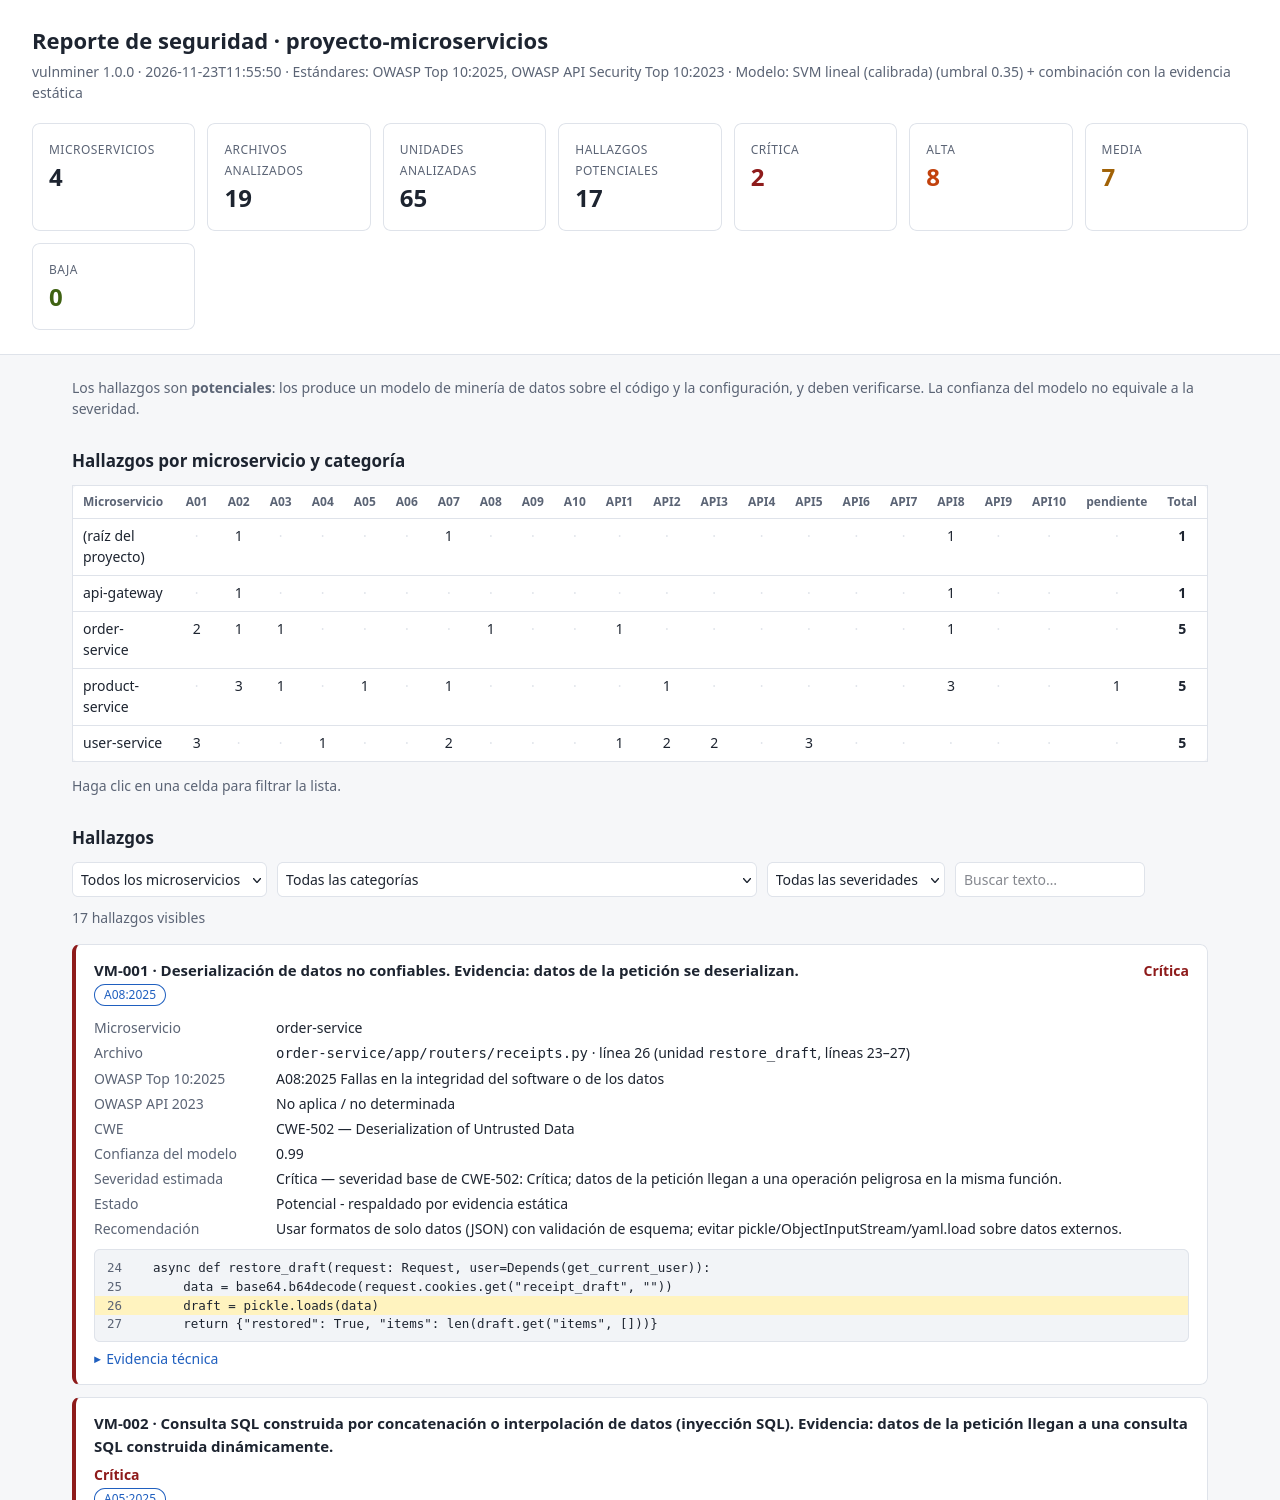
\includegraphics[width=0.92\textwidth]{reporte_html.png}
\caption{Reporte HTML del proyecto de demostración: resumen, matriz microservicio \(\times\) categoría y detalle de un hallazgo.}
\label{fig:html}
\end{figure}

% =========================================================
\section{Evaluación funcional sobre proyectos no vistos}\label{sec:proyectos}
Ejecuté la herramienta completa sobre \nProyectosVulnerables{} proyectos de microservicios vulnerables con vulnerabilidades \textbf{documentadas por sus autores} (OWASP crAPI, VAmPI, dvws-node, Damn Vulnerable RESTaurant y VRPlayground \cite{crapi,vampi,dvws,restaurant,vrplayground}) y sobre dos proyectos de referencia sin vulnerabilidades intencionales (Spring PetClinic Microservices y Online Boutique \cite{petclinic,boutique}). Ninguno participó en el entrenamiento ni en el conjunto de desarrollo. Para cada vulnerabilidad documentada registré el archivo y la línea en \ruta{evaluacion/verdad_terreno.json}; se cuenta como detectada si algún hallazgo cae en la función que la contiene. El proyecto de demostración se informa aparte porque lo escribí yo y, por tanto, sus resultados son una estimación optimista.

\begin{table}[H]
\centering\footnotesize
\caption{Resultados por proyecto: vulnerables, demostración y referencia.}
\label{tab:proyectos}
\setlength{\tabcolsep}{4pt}
\begin{tabularx}{\textwidth}{@{}Yccccccc@{}}
\toprule
\textbf{Proyecto} & \textbf{Serv.} & \textbf{Arch.} & \textbf{Unid.} & \textbf{Hall.} & \textbf{Por 100} & \textbf{Detect.} & \textbf{Categ.}\\
\midrule
\tabla{tabla_proyectos.tex}
\bottomrule
\end{tabularx}
\end{table}

En total, la herramienta detectó \extDetectadas{} de \extDocumentadas{} vulnerabilidades documentadas (sensibilidad \extSensibilidad{}), y en \extCategoria{} casos (\extCategoriaPct{} de las detectadas) la categoría asignada coincidió con alguna de las esperadas. En el proyecto de demostración detectó \demoDetectadas{} de \demoSembradas{}. En los proyectos de referencia, la densidad de hallazgos fue baja en PetClinic y moderada en Online Boutique; más de la mitad de los de Online Boutique señala una mala práctica real de configuración: imágenes base sin versión fijada en los Dockerfile. La Tabla~\ref{tab:cobertura} desglosa el resultado por categoría y demuestra la cobertura funcional exigida: siete categorías del Top 10:2025 y cinco de API Security 2023 se detectaron con la categoría correcta en proyectos no vistos.

\begin{table}[H]
\centering\footnotesize
\caption{Vulnerabilidades documentadas por categoría en los proyectos vulnerables no vistos.}
\label{tab:cobertura}
\begin{tabularx}{\textwidth}{@{}lYccc@{}}
\toprule
\textbf{Código} & \textbf{Categoría} & \textbf{Documentadas} & \textbf{Detectadas} & \textbf{Categoría correcta}\\
\midrule
\tabla{tabla_cobertura_externa.tex}
\bottomrule
\end{tabularx}
\end{table}

\begin{figure}[H]
\centering
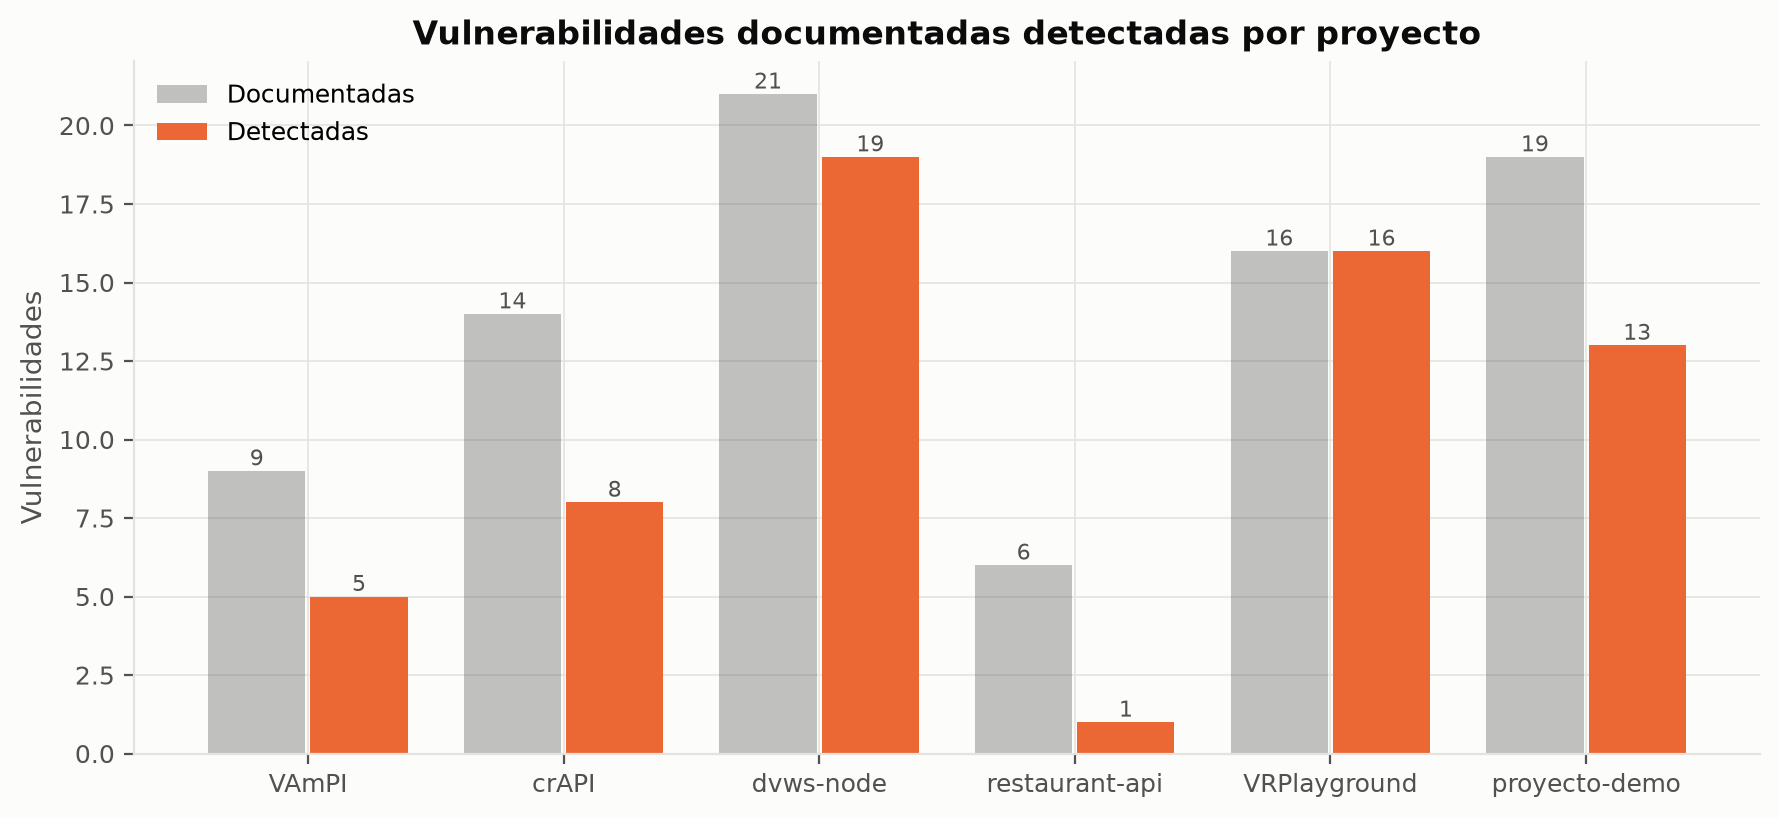
\includegraphics[width=0.85\textwidth]{evaluacion_proyectos.png}
\caption{Vulnerabilidades documentadas y detectadas por proyecto.}
\label{fig:proyectos}
\end{figure}

\textbf{Vulnerabilidades no detectadas.} Casi todas las que no se detectaron son de \textbf{autorización y lógica de negocio}: BOLA en crAPI y RESTaurant, endpoints administrativos sin verificación de rol (API5, ninguna detectada) y exposición de propiedades sensibles (API3). La decisión correcta depende de información que no está en la función, por ejemplo qué rol puede borrar un elemento del menú o qué atributos de un modelo son sensibles. Las demás son patrones casi ausentes del entrenamiento, como la contaminación de prototipo en JavaScript o la exposición de la tecnología en cabeceras HTTP. Bajar el umbral rinde poco: con 0,25 en lugar de \umbral{}, el modelo base detecta cuatro vulnerabilidades más a costa de 18 unidades limpias más marcadas.

% =========================================================
\section{Categorías evaluadas y no evaluadas}
El modelo tiene clasificador para \nCategoriasEvaluadas{} de las 20 categorías. \textbf{API6:2023} (acceso ilimitado a flujos de negocio sensibles) se declara \textbf{no evaluada}: depende de la lógica de negocio de cada aplicación (qué flujo es sensible, qué ritmo de uso es legítimo) y no hay datos etiquetados que permitan aprenderla de forma estática. \textbf{API9:2023} (inventario) tampoco alcanzó el mínimo de ejemplos de entrenamiento y se declara no evaluada; sus patrones (versiones antiguas, servidores de pruebas, documentación expuesta) quedan cubiertos como configuración insegura (A02 y API8). Ambas aparecen como \emph{no evaluadas} en todos los reportes y en el comando \cod{vulnminer info}. Entre las evaluadas, A03, A09, A10 y API5 tienen pocos ejemplos y sus resultados deben leerse con cautela.

% =========================================================
\section{Limitaciones y propuestas de mejora}
\begin{itemize}
  \item \textbf{Análisis estático por unidad.} Cada función se analiza con su contexto inmediato (clase y \emph{middleware} del archivo), pero no se sigue el flujo de datos entre archivos ni entre servicios. Por eso las fallas de autorización (API1, API5) y de lógica de negocio siguen siendo la principal debilidad. \emph{Mejora:} incorporar un grafo de llamadas para relacionar un endpoint con el servicio y el repositorio que usa, y ampliar los ejemplos de autorización en código de producción.
  \item \textbf{Cambio de distribución.} La mayoría de los ejemplos vulnerables proviene de pruebas de reglas y casos de Benchmark, más cortos y artificiales que el código real. La etapa de combinación lo compensa en parte, pero se ajustó con solo \devPositivas{} vulnerabilidades de dos aplicaciones. \emph{Mejora:} ampliar el conjunto de desarrollo con más aplicaciones vulnerables documentadas, por ejemplo con datasets de correcciones reales de vulnerabilidades (CVEfixes) \cite{cvefixes}.
  \item \textbf{Evaluación externa.} Los proyectos de evaluación se usaron en varias rondas de diagnóstico durante el desarrollo (por ejemplo, para detectar que el código de navegador no debía pasar por la combinación). Aunque nunca participaron en el entrenamiento, sus cifras deben leerse como una estimación algo optimista; la partición de prueba sí se usó una sola vez.
  \item \textbf{Categorías con pocos datos.} A03, A09, A10, API5 y API9 tienen pocos ejemplos; API6 no tiene ninguno.
  \item \textbf{Alcance.} Go, C\#, PHP y otros lenguajes se detectan pero no se analizan; se listan como no soportados en el reporte. Los hallazgos son potenciales y requieren verificación, idealmente con pruebas dinámicas (DAST) sobre el entorno desplegado.
\end{itemize}

% =========================================================
\section{Conclusiones}
\begin{itemize}
  \item Respondiendo a la pregunta orientadora: un modelo de minería de datos desarrollado con SEMMA \textbf{sí permite identificar y clasificar} una parte importante de las vulnerabilidades de un proyecto de microservicios. En cinco proyectos vulnerables que no participaron en el entrenamiento, la herramienta detectó \extDetectadas{} de \extDocumentadas{} vulnerabilidades documentadas, con la categoría correcta en \extCategoriaPct{} de las detectadas, y cubrió siete categorías del Top 10:2025 y cinco del API Security Top 10:2023.
  \item La medida en que lo logra depende del tipo de vulnerabilidad. Las que tienen una huella en el código (inyección, deserialización, criptografía débil, secretos, configuración insegura, SSRF) se detectan bien; las de autorización y lógica de negocio, que dependen de reglas del negocio que no están escritas en la función, solo en parte.
  \item El modelo aporta frente a las alternativas sin aprendizaje. Las reglas solas no distinguen un caso vulnerable de su versión corregida (F1 de \ablReglasDesarrolloF{} frente a \ablCompletoF{}) ni clasifican lo que encuentran; en aplicaciones reales la cantidad de evidencia estática es una señal fuerte, y por eso el modelo final la incorpora como variable. Frente a Semgrep con sus reglas comunitarias, la herramienta detectó \sgVulnminer{} vulnerabilidades en lugar de \sgDetectadas{} y, en conjunto, marcó menos código en los proyectos limpios.
  \item La fase Assess fue decisiva. El estudio de ablación reveló que el modelo había aprendido a ignorar la cantidad de evidencia estática por un sesgo de los datos de entrenamiento, y la etapa de combinación ajustada con aplicaciones reales elevó la detección en proyectos reales. Esta iteración entre evaluación y modelado es el aporte práctico de seguir SEMMA en lugar de entrenar una sola vez.
  \item Separar un conjunto de desarrollo de aplicaciones reales fue tan importante como el algoritmo: evitó elegir una representación que solo funcionaba con las fuentes de entrenamiento y permitió calibrar el umbral para que la herramienta sea útil en proyectos reales, con pocas falsas alarmas.
  \item La herramienta es una ayuda para priorizar la revisión, no un sustituto de ella: cada hallazgo es potencial, trae su evidencia y su línea para verificarlo rápidamente, e indica cuándo requiere verificación manual o dinámica.
\end{itemize}

% =========================================================
\begin{thebibliography}{99}
\small
\bibitem{owasp2025} OWASP Foundation. \emph{OWASP Top 10:2025}. \url{https://owasp.org/Top10/2025/}
\bibitem{owaspapi} OWASP Foundation. \emph{OWASP API Security Top 10:2023}. \url{https://owasp.org/API-Security/editions/2023/en/0x11-t10/}
\bibitem{cwe} MITRE Corporation. \emph{Common Weakness Enumeration (CWE)}. \url{https://cwe.mitre.org/}
\bibitem{semma} SAS Institute. \emph{Introduction to SEMMA}. SAS Enterprise Miner documentation.
\bibitem{sklearn} F.~Pedregosa et~al. Scikit-learn: Machine Learning in Python. \emph{Journal of Machine Learning Research}, 12:2825--2830, 2011.
\bibitem{sechidis} K.~Sechidis, G.~Tsoumakas e I.~Vlahavas. On the Stratification of Multi-label Data. En \emph{Machine Learning and Knowledge Discovery in Databases (ECML PKDD)}, pp.~145--158, 2011.
\bibitem{semgrep} Semgrep. \emph{semgrep-rules}. \url{https://github.com/semgrep/semgrep-rules}
\bibitem{semgreptool} Semgrep. \emph{Semgrep: lightweight static analysis}. \url{https://github.com/semgrep/semgrep}
\bibitem{codeql} GitHub. \emph{CodeQL}. \url{https://github.com/github/codeql}
\bibitem{benchmark} OWASP Foundation. \emph{OWASP Benchmark}. \url{https://owasp.org/www-project-benchmark/}
\bibitem{kics} Checkmarx. \emph{KICS: Keeping Infrastructure as Code Secure}. \url{https://github.com/Checkmarx/kics}
\bibitem{securityeval} M.~L. Siddiq y J.~C.~S. Santos. SecurityEval Dataset. En \emph{Proceedings of MSR4P\&S}, 2022. \url{https://github.com/s2e-lab/SecurityEval}
\bibitem{juiceshop} OWASP Foundation. \emph{OWASP Juice Shop}. \url{https://github.com/juice-shop/juice-shop}
\bibitem{vulnerableapp} OWASP Foundation. \emph{OWASP VulnerableApp}. \url{https://github.com/SasanLabs/VulnerableApp}
\bibitem{pygoat} OWASP Foundation. \emph{OWASP PyGoat}. \url{https://github.com/adeyosemanputra/pygoat}
\bibitem{nodegoat} OWASP Foundation. \emph{OWASP NodeGoat}. \url{https://github.com/OWASP/NodeGoat}
\bibitem{realworld} RealWorld. \emph{RealWorld example apps}. \url{https://github.com/gothinkster/realworld}
\bibitem{robotshop} Instana. \emph{Robot Shop}. \url{https://github.com/instana/robot-shop}
\bibitem{ftgo} C.~Richardson. \emph{FTGO application}. \url{https://github.com/microservices-patterns/ftgo-application}
\bibitem{crapi} OWASP Foundation. \emph{completely ridiculous API (crAPI)}. \url{https://github.com/OWASP/crAPI}
\bibitem{vampi} erev0s. \emph{VAmPI: Vulnerable REST API}. \url{https://github.com/erev0s/VAmPI}
\bibitem{dvws} snoopysecurity. \emph{Damn Vulnerable Web Services (dvws-node)}. \url{https://github.com/snoopysecurity/dvws-node}
\bibitem{restaurant} theowni. \emph{Damn Vulnerable RESTaurant API Game}. \url{https://github.com/theowni/Damn-Vulnerable-RESTaurant-API-Game}
\bibitem{vrplayground} F5 DevCentral. \emph{VRPlayground}. \url{https://github.com/f5devcentral/VRPlayground}
\bibitem{petclinic} Spring PetClinic. \emph{Spring PetClinic Microservices}. \url{https://github.com/spring-petclinic/spring-petclinic-microservices}
\bibitem{boutique} Google Cloud Platform. \emph{Online Boutique (microservices-demo)}. \url{https://github.com/GoogleCloudPlatform/microservices-demo}
\bibitem{cvefixes} G.~Bhandari, A.~Naseer y L.~Moonen. CVEfixes: Automated Collection of Vulnerabilities and Their Fixes from Open-Source Software. En \emph{PROMISE}, 2021.
\end{thebibliography}

% =========================================================
\appendix
\section{Trazabilidad de los requerimientos}
\begin{table}[H]
\centering\footnotesize
\caption{Cumplimiento de los requerimientos funcionales.}
\label{tab:requisitos}
\begin{tabularx}{\textwidth}{@{}lP{4.3cm}Y@{}}
\toprule
\textbf{Código} & \textbf{Requerimiento} & \textbf{Evidencia}\\
\midrule
RF01 & Dataset de código vulnerable y no vulnerable & \ruta{datos/dataset.csv} (\nUnidades{} unidades, \nSeguras{} no vulnerables); \ruta{scripts/construir_dataset.py}\\
RF02 & Cinco fases de SEMMA & Notebooks \ruta{01_sample} a \ruta{05_assess} y secciones 4 a 8 de este informe\\
RF03 & Al menos dos algoritmos comparados & Cuatro algoritmos con búsqueda de hiperparámetros (Tablas~\ref{tab:detector} y \ref{tab:categorizador}); \ruta{resultados/comparacion_*.csv}\\
RF04 & Análisis estático de código y configuración & \nIndicadores{} indicadores y \nDerivadas{} interacciones (\ruta{vulnminer/caracteristicas.py}) como variables y evidencia; contribución medida en la sección~\ref{sec:contribucion}\\
RF05 & Clasificación OWASP 2025 y API 2023 & Clasificador multietiqueta con umbral por categoría; categorías no evaluadas declaradas\\
RF06 & Identificación de microservicios & \ruta{vulnminer/descubrimiento.py} (manifiestos, Dockerfile y docker-compose)\\
RF07 & CLI desde el directorio raíz & \cod{vulnminer scan .} (\ruta{vulnminer/cli.py})\\
RF08 & Microservicio, archivo y ubicación & Cada hallazgo informa microservicio, archivo, línea y rango de la unidad\\
RF09 & Reportes JSON y HTML & \ruta{ejemplos/reporte_demo/analisis.json} y \ruta{analisis.html}\\
RF10 & Evaluación con métricas y proyectos no vistos & Partición de prueba, F1 macro, matrices de confusión, siete proyectos de microservicios y comparación con Semgrep (secciones 8 y 10)\\
\bottomrule
\end{tabularx}
\end{table}

Las pruebas automáticas del repositorio (\cod{pytest}) verifican el catálogo y las correspondencias, la segmentación, las características, el dataset (mínimos y ausencia de fugas), el descubrimiento de microservicios, la severidad, la etapa de combinación y la CLI completa, incluidos los casos límite: carpeta sin archivos soportados, archivos binarios, demasiado grandes o sin permiso de lectura, umbral fuera de rango y modelo inexistente.

\section{Detalle de la evaluación en proyectos no vistos}
{\footnotesize
\begin{longtable}{@{}lP{5.6cm}P{2.3cm}cP{0.7cm}P{2.4cm}@{}}
\caption{Vulnerabilidades documentadas y resultado de la herramienta.}\label{tab:detalle}\\
\toprule
\textbf{Id} & \textbf{Vulnerabilidad} & \textbf{Esperado} & \textbf{Det.} & \textbf{Conf.} & \textbf{Categorías predichas}\\
\midrule
\endfirsthead
\toprule
\textbf{Id} & \textbf{Vulnerabilidad} & \textbf{Esperado} & \textbf{Det.} & \textbf{Conf.} & \textbf{Categorías predichas}\\
\midrule
\endhead
\tabla{tabla_detalle_externo.tex}
\bottomrule
\end{longtable}
}

\end{document}
